\documentclass[a4paper]{article}
\usepackage[utf8]{inputenc}
\usepackage{graphicx}
\usepackage{amsmath}
\usepackage{amssymb}
\usepackage{amsfonts}
\usepackage{textcomp}
\usepackage{amsthm}
\usepackage{subcaption}
\usepackage{booktabs}
\usepackage{float}
\usepackage{mathtools}
\usepackage{xfrac}
\usepackage{hyperref}
\usepackage{xfrac}
\usepackage{cancel}
\usepackage[portuguese]{babel}
\usepackage[linguistics]{forest}
\DeclareMathOperator{\tr}{tr}
\DeclareMathOperator{\aut}{Aut}
\DeclareMathOperator{\inn}{Inn}
\DeclareMathOperator{\stab}{stab}
\DeclareMathOperator{\orb}{orb}
\DeclareMathOperator{\Mod}{Mod}
\DeclareMathOperator{\Ker}{Ker}
\usepackage{anonchap}
\usepackage[symbol]{footmisc}
\usepackage{anonchap}
\usepackage[Sonny]{fncychap}
%\usepackage[brazilian]{babel}
%\usepackage[portuguese]{babel}
\usepackage{geometry}
\geometry{a4paper, left=3cm, top=3cm, right=2cm, bottom=2cm}
\usepackage{multicol}
\usepackage{fancyhdr}
\newtheorem{theorem}{Teorema}[section]
\newtheorem*{definition}{Definição}
\newtheorem{corollary}{Corolário}[theorem]
\newtheorem{lemma}[theorem]{Lema}
\newtheorem{remark}{Observação}[section]
\newtheorem{deff}{Definição}[section]
\newtheorem{fact}{Fato}[section]
\newtheorem{exercise}{Exercício}[section]
\newtheorem{example}{Exemplo}[section]
\newtheorem{prop}{Proposição}[section]
\newtheorem*{solution}{Solução}

\title{Soluções}
\date{}
\author{Caio Tomás}

\begin{document}
	\maketitle
	\tableofcontents
	\newpage
	\section{Estatística}
	\begin{figure}[H]
		\begin{center}
			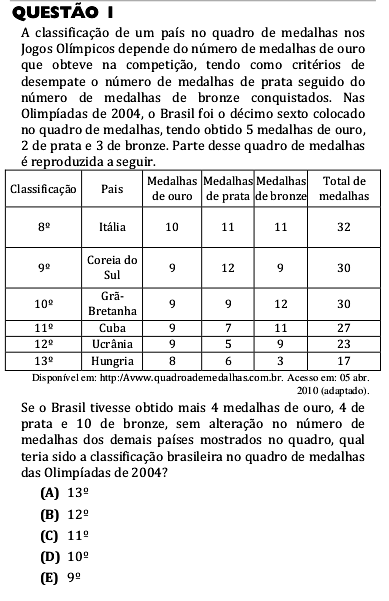
\includegraphics[width=8cm]{L1Q1.png}
		\end{center}
	\end{figure}
\par\textbf{(Gabarito: B)} Do texto, sabemos que o Brasil obteve 5 medalhas de ouro, 2 de prata e 3 de bronze. Se o Brasil tivesse obtido mais 4 medalhas de ouro, 4 de prata e 10 de bronze, ele teria, no total, 9 medalhas de ouro (as 5 iniciais mais as outras 4), 6 de prata (as 2 iniciais mais as outras 4) e 13 de bronze (as 3 iniciais mais as outras 10).
\par\vspace{0.3cm} Olhando a tabela, vemos que a Hungria obteve apenas 8 medalhas de ouro. Logo, como a quantidade de medalhas de ouro é o primeiro critério de classificação, o Brasil fica à frente da Hungria. Também da tabela, vemos que a Ucrânia obteve 9 medalhas de ouro, número igual ao Brasil. Então, vamos olhar a quantidade de medalhas de prata, o primeiro critério de desempate. A Ucrânia tem 5 medalhas de prata, e o Brasil, 6. Logo, o Brasil fica à frente da Ucrânia. Por último, como Cuba também tem 9 medalhas de ouro, vamos olhar a quantidade de medalhas de prata. Cuba tem 7, o Brasil, 6. Portanto, o Brasil fica logo atrás de Cuba, ou seja, em $12^{\circ}$ lugar. 
\begin{figure}[H]
	\begin{center}
		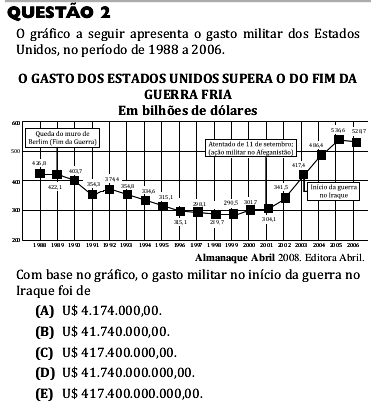
\includegraphics[width=9cm]{L1Q2.png}
	\end{center}
\end{figure}
\par \textbf{(Gabarito: E)} Do gráfico, o gasto militar no início da Guerra do Iraque foi de U\$ $417,4$ bilhões. Como $1$ bilhão de dólares $= 10^9$ dólares, então $417,4$ bilhões $= 417,4\times 10^9 = 417.400.000.000,00$ dólares.
\begin{figure}[H]
	\begin{center}
		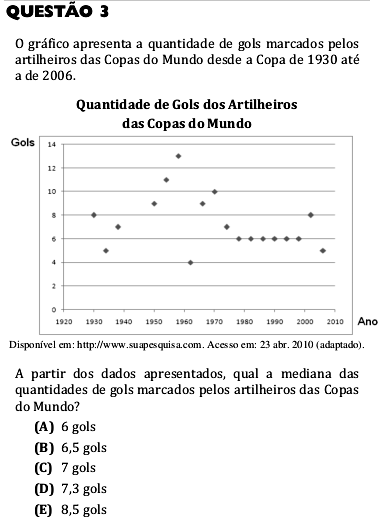
\includegraphics[width=9cm]{L1Q3.png}
	\end{center}
\end{figure}
\par \textbf{(Gabarito: B)} Lembre que a mediana é o "valor do meio" de uma distribuição de dados. Contudo, essa distribuição deve estar organizada em ordem crescente: precisamos fazer o rol. 
\par\vspace{0.3cm} Do gráfico, temos $18$ valores para organizar. Fazendo o rol, temos o seguinte:
\begin{equation*}
4, 5, 5, 6, 6, 6, 6, 6, 6, 7, 7, 8, 8, 9, 9, 10, 11, 13
\end{equation*}
\par\vspace{0.3cm} Como a quantidade de elementos da nossa distribuição é par, a mediana será dada pela média aritmética dos dois termos "do meio". Nesse caso, os dois termos do meio são o $9^\circ$ e o $10^\circ$, que valem, respectivamente, $6$ e $7$. Fazendo a média, temos que a mediana dessa distribuição vale $6,5$.
\begin{figure}[H]
	\begin{center}
		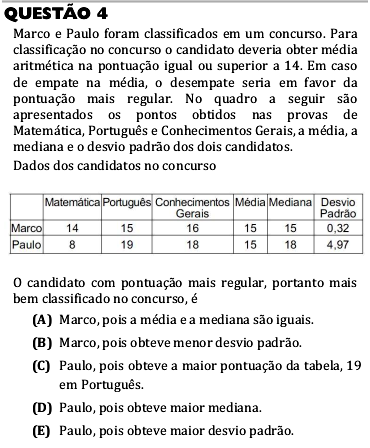
\includegraphics[width=9cm]{L1Q4.png}
	\end{center}
\end{figure}
\par \textbf{(Gabarito: B)} Nessa questão é importante reconhecer que \textbf{pontuação mais regular} corresponde a \textbf{menor desvio padrão}, pois o desvio padrão mede exatamente isso: o quanto a distribuição se desvia, se espalha, em relação à média. Um desvio padrão menor significa que os valores da distribuição não são muito diferentes da média, enquanto que um desvio padrão maior significa que os valores da distribuição diferem bastante da média.
\par\vspace{0.3cm} Da tabela, vemos que Marco e Paulo tiveram a mesma média. Nesse caso, o desempate é em favor do candidato com pontuação mais regular. Olhando para os desvios padrão de Marco e Paulo, podemos ver que Marco obteve a pontuação mais regular, pois seu desvio padrão é o menor.
\begin{figure}[H]
	\begin{center}
		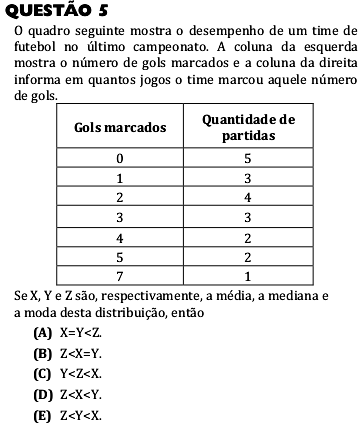
\includegraphics[width=9cm]{L1Q5.png}
	\end{center}
\end{figure}
\par\textbf{(Gabarito: E)} A tabela nos dá a seguinte distribuição:
\begin{equation*}
0,0,0,0,0,1,1,1,2,2,2,2,3,3,3,4,4,5,5,7
\end{equation*}
\par\vspace{0.3cm} Daí, a média é
\begin{equation*}
X = \frac{0+0+0+0+0+1+1+1+2+2+2+2+3+3+3+4+4+5+5+7}{5+3+4+3+2+2+1} = \frac{45}{20} = 2,25
\end{equation*}
\par\vspace{0.3cm} A mediana, como temos uma quantidade par de dados, será dada pela média aritmética do $10^\circ$ com o $11^\circ$ termo. Como ambos são iguais a $2$, a média é
\begin{equation*}
Y = \frac{2+2}{2} = \frac{4}{2} = 2
\end{equation*}
\par\vspace{0.3cm} Por fim, a moda é o valor mais frequente da distribuição, o valor que mais aparece. Podemos ver, tanto da tabela quanto da distribuição, que o valor que mais aparece é o $0$, aparecendo $5$ vezes. Portanto, a moda é $Z = 0$.
\par\vspace{0.3cm} Daí, podemos ver que $Z<Y<X$.
\begin{figure}[H]
	\begin{center}
		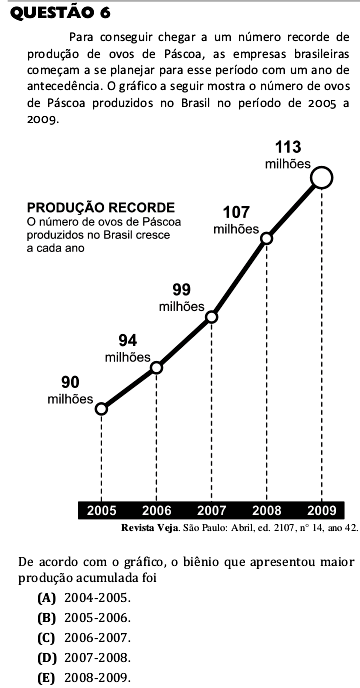
\includegraphics[width=8cm]{L1Q6.png}
	\end{center}
\end{figure}
\par\textbf{(Gabarito: E)} Queremos encontrar o biênio com a maior produção acumulada, ou seja, os dois anos consecutivos cujas produções somadas é a maior. Do gráfico, podemos ver que a maior soma será $107+113$, correspondente ao biênio $2008$-$2009$.
\begin{figure}[H]
	\begin{center}
		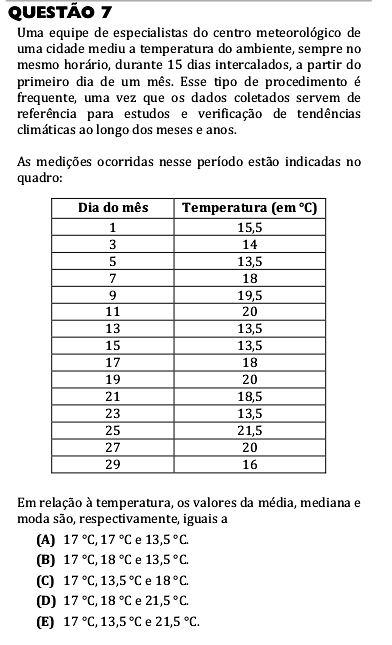
\includegraphics[width=8cm]{L1Q7.png}
	\end{center}
\end{figure}
\par\textbf{(Gabarito: B)} Antes de escrever a distribuição, note que em todas as opções a média é $17^\circ$C. Portanto, poderíamos resolver a questão sem calcular a média. A nossa distribuição, já organizada em ordem crescente, é
\begin{equation*}
13,5; 13,5; 13,5; 13,5; 14; 15,5; 16; 18; 18; 18,5; 19,5; 20; 20; 20; 21,5 
\end{equation*}
\par\vspace{0.3cm} A mediana será dada pelo termo do meio, que nesse caso é o $8^\circ$ termo, ou seja, $18^\circ$C. Além disso, vemos que o valor mais frequente, que aparece mais, é $13,5^\circ$C, logo a moda é $13,5^\circ$C.
\par\vspace{0.3cm} Apesar de não ser necessário para resolver a questão, vamos calcular a média. Usando a distribuição acima, temos que a média é
\begin{equation*}
\frac{13,5+13,5+13,5+13,5+14+15,5+16+18+18+18,5+19,5+20+20+21,5}{15} = \frac{255}{15} = 17
\end{equation*}
\begin{figure}[H]
	\begin{center}
		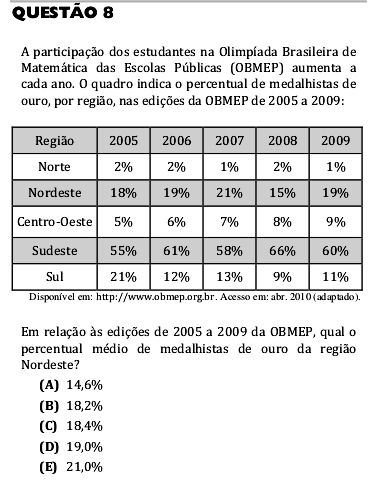
\includegraphics[width=9cm]{L1Q8.png}
	\end{center}
\end{figure}
\par\textbf{(Gabarito: C)} Queremos encontrar o percentual médio de medalhistas de ouro da região Nordeste entre as edições de $2005$ a $2009$. Para isso, basta fazer a média aritmética dos valores de $2005$ a $2009$, obtendo:
\begin{equation*}
\frac{18\%+19\%+21\%+15\%+19\%}{5} = \frac{92\%}{5} = 18,4\%
\end{equation*}
\begin{figure}[H]
	\begin{center}
		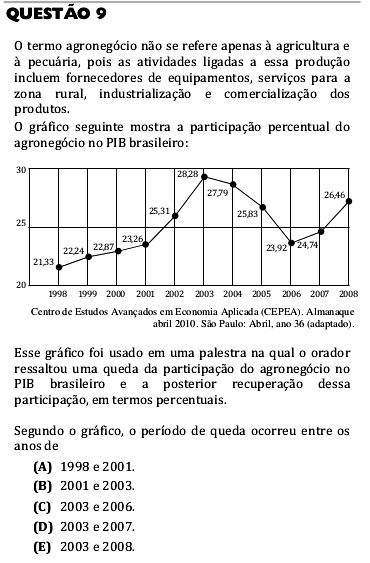
\includegraphics[width=9cm]{L1Q9.png}
	\end{center}
\end{figure}
\par\textbf{(Gabarito: C)} Do gráfico, podemos ver que entre os anos de $2003$ a $2006$ a participação do agronegócio no PIB brasileiro só diminuiu: de $28,28\%$ em $2003$ para $27,79\%$ em $2004$ para $25,83\%$ em $2005$ para $23,92\%$ em $2006$.
\begin{figure}[H]
	\begin{center}
		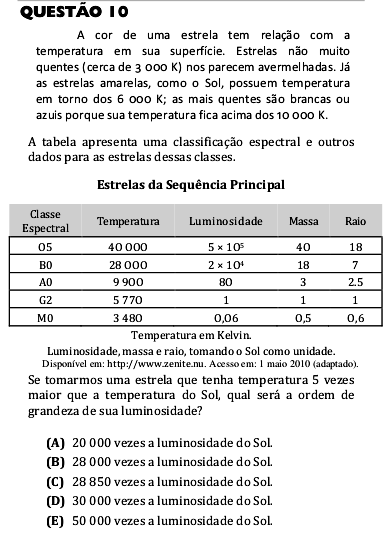
\includegraphics[width=9cm]{L1Q10.png}
	\end{center}
\end{figure}
\par\textbf{(Gabarito: A)} Do texto, sabemos que a temperatura do Sol está em torno de $6000$ K. Logo, da tabela, sabemos que o Sol pertence à classe espectral G$2$, com luminosidade igual a $1$. Uma estrela com $5$ vezes a temperatura do Sol tem temperatura em torno de $30\ 000$ K. Portanto, da tabela, sabemos que essa estrela pertence à classe espectral B$0$, com luminosidade $2\times10^4 = 20\ 000$. Portanto, como a luminosidade do Sol é igual a $1$, essa estrela tem luminosidade igual $\displaystyle{ \frac{20\ 000}{1} = 20\ 000}$ vezes a do Sol.
\begin{figure}[H]
	\begin{center}
		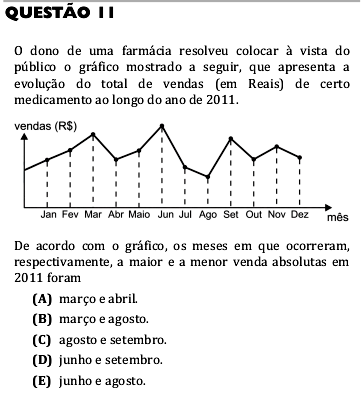
\includegraphics[width=9cm]{L1Q11.png}
	\end{center}
\end{figure}
\par\textbf{(Gabarito: E)} Do gráfico, vemos que o ponto mais alto ocorreu em Junho, enquanto que o ponto mais baixo ocorreu em Agosto.
\begin{figure}[H]
	\begin{center}
		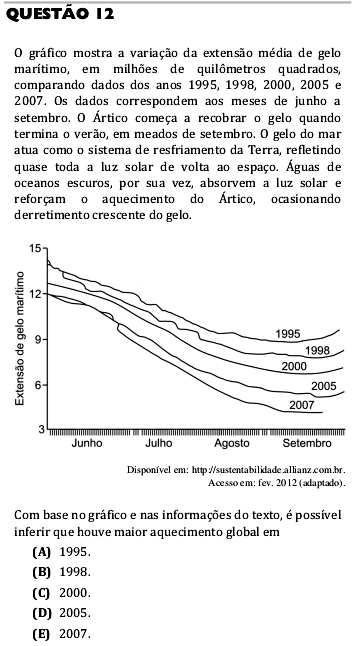
\includegraphics[width=9cm]{L1Q12.png}
	\end{center}
\end{figure}
\par\textbf{(Gabarito: E)} Pelas informações do texto, sabemos que o gelo do mar atua como sistema de resfriamento da Terra, refletindo quase toda a luz solar. Consequentemente, quanto menos gelo há, maior o aquecimento global. A partir do gráfico, vemos que no ano de $2007$ a extensão de gelo marítimo foi a menor. Portanto, em $2007$ houve o maior aquecimento global.
\begin{figure}[H]
	\begin{center}
		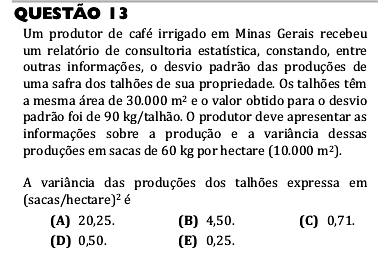
\includegraphics[width=10cm]{L1Q13.png}
	\end{center}
\end{figure}
\par\textbf{(Gabarito: E)} Queremos descobrir a variância, expressa em $(\text{sacas}/\text{hectare})^2$. Lembre-se que a variância é dada pelo quadrado do desvio padrão. Do texto, sabemos que o desvio padrão é de $90\text{ kg}/\text{talhão}$. Também sabemos que uma saca tem $60$ kg, que um talhão tem $30\ 000$ m$^2$ e que um hectare tem $10\ 000$ m$^2$. 
\par\vspace{0.3cm} Como $60$ kg correspondem a $1$ saca, então $90$ kg correspondem a $1,5$ sacas. De modo semelhante, como $10\ 000$ m$^2$ correspondem a $1$ hectare, então $30\ 000$ m$^2$ correspondem a $3$ hectares. Logo, o desvio padrão é igual a
\begin{equation*}
\frac{90\text{ kg}}{1\text{ talhão}} = \frac{1,5\text{ sacas}}{30\ 000\text{ m}^2} = \frac{1,5\text{ sacas}}{3\text{ hectares}} = 0,5\text{ sacas}/\text{hectare}
\end{equation*} 
\par\vspace{0.3cm} Elevando esse valor ao quadrado, obtemos que a variância é igual a
\begin{equation*}
0,25\ (\text{sacas}/\text{hectare})^2
\end{equation*}
\begin{figure}[H]
	\begin{center}
		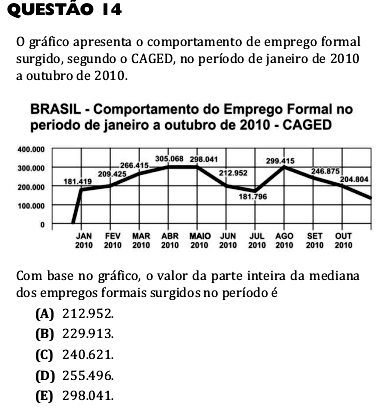
\includegraphics[width=12cm]{L1Q14.png}
	\end{center}
\end{figure}
\par\textbf{(Gabarito: B)} Queremos encontrar a mediana da distribuição mostrada no gráfico. Para isso, vamos organizar os valores em ordem crescente, ou seja, fazer o rol:
\begin{equation*}
181.419, 181.796, 204.804, 209.425, 212.952, 246.875, 266.415, 298.041, 299.415, 305.068
\end{equation*}
\par\vspace{0.3cm} Como a distribuição tem $10$ valores, a mediana será dada pela média aritmética do $5^\circ$ com o $6^\circ$ termo. Calculando, temos:
\begin{equation*}
\frac{212.952 + 246.875}{2} = \frac{459.827}{2} = 229.913,5
\end{equation*}
\par\vspace{0.3cm} Desconsiderando a parte decimal, a parte inteira da mediana é $229.913$.
\begin{figure}[H]
	\begin{center}
		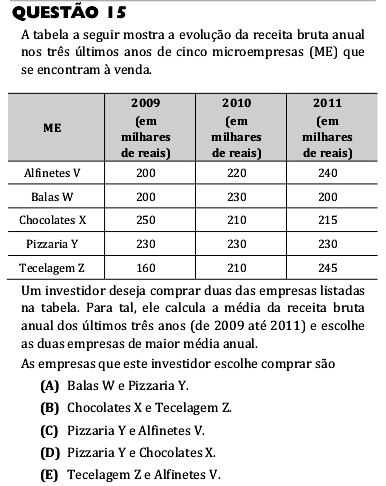
\includegraphics[width=10cm]{L1Q15.png}
	\end{center}
\end{figure}
\par\textbf{(Gabarito: D)} Queremos encontrar as duas microempresas que têm a maior média de receita bruta nos três últimos anos. Note, contudo, que não precisamos calcular a média de todas as empresas. Podemos apenas somar as receitas dos três últimos anos e comparar as somas, pois quanto maior a soma, maior será a média. Desse modo, temos os seguintes valores:
\begin{align*}
\text{Alfinetes V: }200+220+240 = 660 \\
\text{Balas W: }200+230+200 = 630 \\
\text{Chocolates X: }250+210+215 = 675 \\
\text{Pizzaria Y: }230+230+230 = 690 \\
\text{Tecelagem Z: }160+210+245 = 615
\end{align*}
\par\vspace{0.3cm} Podemos ver que Pizzaria Y e Chocolates X foram as duas microempresas com a maior soma e, consequentemente, a maior média de receita bruta nos três últimos anos. 
\begin{figure}[H]
	\begin{center}
		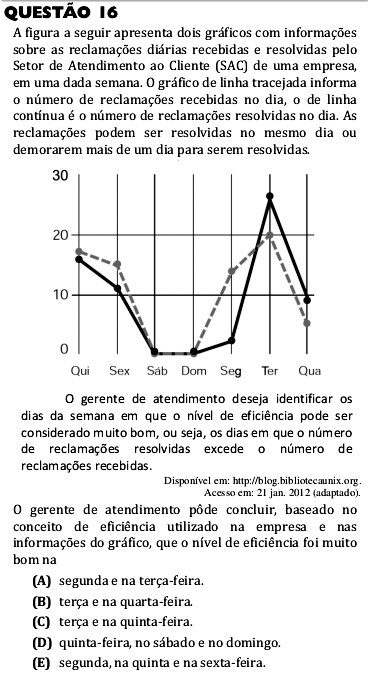
\includegraphics[width=10cm]{L1Q16.png}
	\end{center}
\end{figure}
\par\textbf{(Gabarito: B)} Queremos saber os dias em que o número de reclamações resolvidas (linha contínua) excede o número de reclamações recebidas (linha tracejada), ou seja, queremos saber os dias em que a linha contínua está acima da linha tracejada. Do gráfico, vemos que isso ocorre na terça e quarta-feira.
\begin{figure}[H]
	\begin{center}
		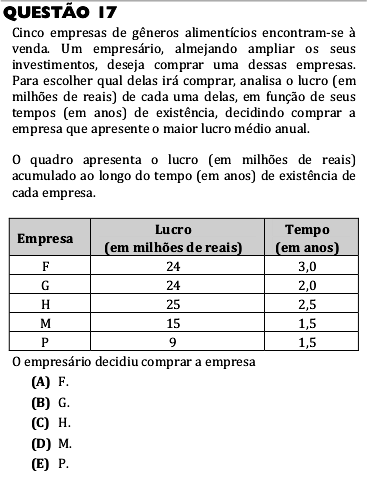
\includegraphics[width=9cm]{L1Q17.png}
	\end{center}
\end{figure}
\par\textbf{(Gabarito: B)} Queremos encontrar a empresa com maior lucro médio anual. Chamando de $LM_F$ o lucro médio anual da empresa $F$, temos os seguintes valores:
\begin{align*}
LM_F = \frac{24}{3} =  8 \\
LM_G = \frac{24}{2} =  12 \\
LM_H = \frac{25}{2,5} =  10 \\
LM_M = \frac{15}{1,5} =  10 \\
LM_P = \frac{9}{1,5} =  6 \\
\end{align*}
\par\vspace{0.3cm} Daí, podemos ver que a empresa $G$ foi a que obteve o maior lucro médio anual.
\begin{figure}[H]
	\begin{center}
		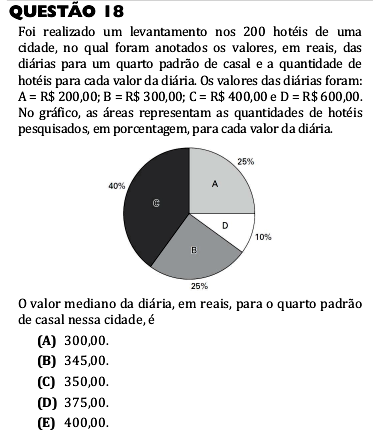
\includegraphics[width=10cm]{L1Q18.png}
	\end{center}
\end{figure}
\par\textbf{(Gabarito: C)} Queremos encontrar a mediana da distribuição de preços de diárias dos hotéis. Como há $200$ hotéis, ou seja, $200$ valores nessa distribuição, a mediana será dada pela média aritmética do $100^\circ$ com o $101^\circ$ termo (colocando todos os termos em ordem crescente).
\par\vspace{0.3cm} Do gráfico, sabemos que há as seguintes quantidades de hotéis para cada valor de diária:
\begin{align*}
\text{A: }200\times 0,25 = 50 \\
\text{B: }200\times 0,25 = 50 \\
\text{C: }200\times 0,4 = 80 \\
\text{D: }200\times 0,1 = 20
\end{align*}
\par\vspace{0.3cm} Consequentemente, o $100^\circ$ termo será a diária de R\$ 300,00 e o $101^\circ$ será a diária de R\$ 400,00. Fazendo a média, temos que a mediana será:
\begin{equation*}
\frac{\text{R\$}300+\text{R\$}400}{2} = \text{R\$}350,00 
\end{equation*}
\begin{figure}[H]
	\begin{center}
		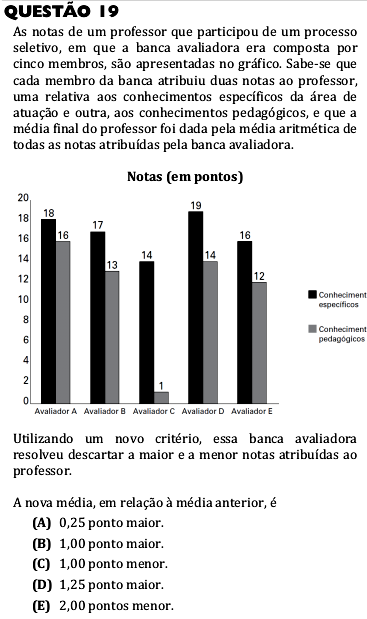
\includegraphics[width=9.5cm]{L1Q19.png}
	\end{center}
\end{figure}
\par\textbf{(Gabarito: B)} A média inicial é igual a 
\begin{equation*}
\frac{18+16+17+13+14+1+19+14+16+12}{10} = \frac{140}{10} = 14
\end{equation*}
\par\vspace{0.3cm} Para a nova média, descartamos a maior e a menor nota. Logo, a soma será $140-19-1 = 120$. Como descartamos dois valores, nos restaram apenas $8$. Portanto, a nova média é igual a
\begin{equation*}
\frac{120}{8} = 15
\end{equation*}
\par\vspace{0.3cm} sendo $1,00$ ponto maior que a média anterior.
\begin{figure}[H]
	\begin{center}
		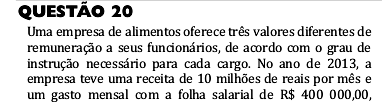
\includegraphics[width=9.5cm]{L1Q20_1.png}
	\end{center}
\end{figure}
\begin{figure}[H]
	\begin{center}
		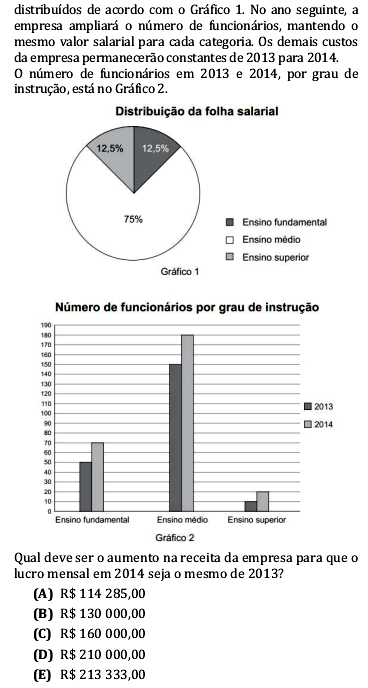
\includegraphics[width=9.5cm]{L1Q20_2.png}
	\end{center}
\end{figure}
\par\textbf{(Gabarito: B)} Queremos saber qual deve ser o aumento na receita da empresa para que o lucro mensal de $2014$ seja o mesmo de $2013$. Sabemos que, em $2013$, o gasto com a folha salarial foi de R\$ $400\ 000,00$. Do gráfico de pizza, sabemos a distribuição da folha salarial enter as três categorias. Com isso, podemos calcular quanto é gasto em cada categoria, da seguinte forma:
\begin{align*}
\text{Ensino Fundamental: }12,5\%\times \text{R\$}400\ 000 &= \text{R\$}50\ 000 \\ 
\text{Ensino Médio: }75\%\times \text{R\$}400\ 000 &= \text{R\$}300\ 000 \\
\text{Ensino Superior: }12,5\%\times \text{R\$}400\ 000 &= \text{R\$}50\ 000 
\end{align*}
\par\vspace{0.3cm} Com o gráfico de barras, podemos calcular o salário de cada categoria, da seguinte forma:
\begin{align*}
\text{Salário EF: } \frac{\text{R\$50\ 000}}{50} = \text{R\$}1000 \\
\text{Salário EM: } \frac{\text{R\$300\ 000}}{150} = \text{R\$}2000 \\
\text{Salário ES: } \frac{\text{R\$50\ 000}}{10} = \text{R\$}5000 
\end{align*}
\par\vspace{0.3cm} Do texto, sabemos que o valor salarial de cada categoria se mantém o mesmo em $2014$. Então, usando novamente o gráfico de barras, podemos calcular o gasto da empresa com a folha salarial em $2014$, do seguinte modo:
\begin{align*}
\text{Ensino Fundamental: }70\times \text{R\$}1000 &= \text{R\$}70\ 000 \\ 
\text{Ensino Médio: }180\times \text{R\$}2000 &= \text{R\$}360\ 000 \\
\text{Ensino Superior: }20\times \text{R\$}5000 &= \text{R\$}100\ 000 
\end{align*}
\par\vspace{0.3cm} Portanto, em $2014$, o gasto com a folha salarial é de R\$$70\ 000$ + R\$$360\ 000$ + R\$$100\ 000 = $ R\$$530\ 000$. Então, é necessário um aumento de R\$$530\ 000 - \text{R\$}400\ 000 = \text{R\$}130\ 000$.
\begin{figure}[H]
	\begin{center}
		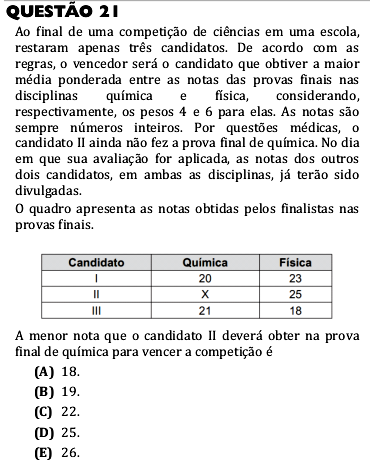
\includegraphics[width=10cm]{L1Q21.png}
	\end{center}
\end{figure}
\par\textbf{(Gabarito: A)} As médias de cada candidato, considerando os pesos de cada prova, são as seguintes:
\begin{align*}
\text{I: }\frac{4\times 20 + 6\times 23}{10} &= \frac{218}{10} = 21,8 \\
\text{II: }\frac{4\times X + 6\times 25}{10} &= \frac{4X + 150}{10} \\
\text{III: }\frac{4\times 21 + 6\times 18}{10} &= \frac{192}{10} = 19,2
\end{align*}
\par\vspace{0.3cm} Queremos encontrar o menor valor de $X$ tal que a média do candidato II seja maior que a média do candidato I, ou seja:
\begin{align*}
\frac{4X + 150}{10} > 21,8 \implies 4X + 150 > 218 \implies 4X > 68 \implies X> 17
\end{align*}
\par\vspace{0.3cm} Portanto, o menor valor de $X$ que permite que o candidato II  vença a competição é $18$.
\begin{figure}[H]
	\begin{center}
		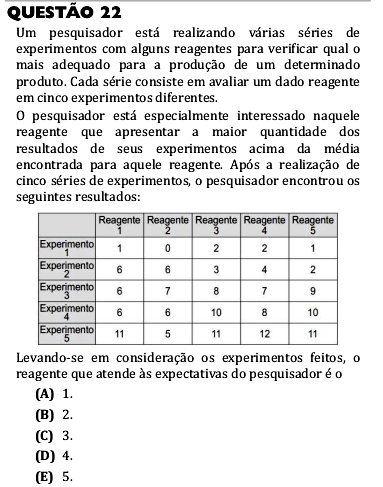
\includegraphics[width=10cm]{L1Q22.png}
	\end{center}
\end{figure}
\par\textbf{(Gabarito: B)} Vamos calcular a média de cada reagente:
\begin{align*}
\text{Reagente 1: }\frac{1 + 6 + 6 + 6 + 11}{5} = \frac{30}{5} &= 6 \\
\text{Reagente 2: }\frac{0 + 6 + 7 + 6 + 5}{5} = \frac{24}{5} &= 4,8 \\
\text{Reagente 3: }\frac{2 + 3 + 8 + 10 + 11}{5} = \frac{34}{5} &= 6,8 \\
\text{Reagente 4: }\frac{2 + 4 + 7 + 8 + 12}{5} = \frac{33}{5} &= 6,6 \\
\text{Reagente 5: }\frac{1 + 2 + 9 + 10 + 11}{5} = \frac{33}{5} &= 6,6 
\end{align*}
\par\vspace{0.3cm} Daí, a quantidade de resultados acima da média para cada reagente são:
\begin{align*}
\text{Reagente 1: }1 \\
\text{Reagente 2: }4 \\
\text{Reagente 3: }3 \\
\text{Reagente 4: }3 \\
\text{Reagente 5: }3 \\
\end{align*}
\par\vspace{0.3cm} Portanto, o reagente 2 deve ser escolhido.
\begin{figure}[H]
	\begin{center}
		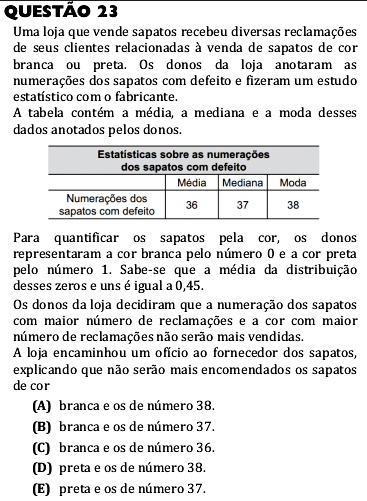
\includegraphics[width=10cm]{L1Q23.png}
	\end{center}
\end{figure}
\par\textbf{(Gabarito: A)} Do texto, sabemos que a média da distribuição de zeros (cor branca) e uns (cor preta) é de $0,45$. Se chamarmos de $B$ a quantidade de sapatos da cor branca e $P$ a quantidade de sapatos da cor preta, temos o seguinte:
\begin{align*}
&\frac{ \overbrace{0+0+\cdots+0}^{B} + \overbrace{1+1+\cdots+1}^{P}}{B+P} = 0,45 \\
&\iff  P = 0,45B + 0,45P \\ 
&\iff 0,55P = 0,45B \\
&\iff B = \frac{0,55}{0,45}P = \frac{11}{9}P > P
\end{align*}
\par\vspace{0.3cm} Então, a quantidade de reclamações de sapatos da cor branca ($B$) é maior que a quantidade de reclamações de sapatos da cor preta ($P$). Logo, os donos da loja devem parar de vender os sapatos com cor branca. Temos agora de descobrir qual a numeração desses sapatos.
\par\vspace{0.3cm} Do texto, sabemos que a numeração com o maior número de reclamações deve ser removida. Olhando a tabela, vemos que a moda dos dados das reclamações anotadas pelos donos é $38$. Lembre que a moda de uma distribuição é o valor que mais aparece nessa distribuição, ou seja, o valor mais frequente. Desse modo, os donos devem para de vender sapatos brancos e de número $38$.
\begin{figure}[H]
	\begin{center}
		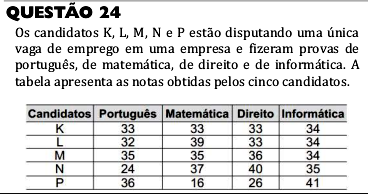
\includegraphics[width=10cm]{L1Q24_1.png}
	\end{center}
\end{figure}
\begin{figure}[H]
	\begin{center}
		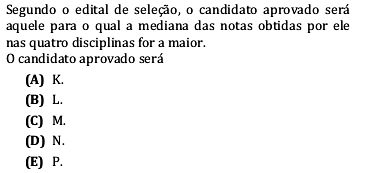
\includegraphics[width=10cm]{L1Q24_2.png}
	\end{center}
\end{figure}
\par\textbf{(Gabarito: D)} Para encontrar a mediana, devemos primeiro organizar os dados de cada candidato em ordem crescente:
\begin{align*}
\text{K:} 33, 33, 33, 34 \\
\text{L: } 32, 33, 34, 39 \\
\text{M: } 34, 35, 35, 36 \\
\text{N: }24, 35, 37, 40 \\
\text{P: }16, 26, 36, 41
\end{align*}
\par\vspace{0.3cm} Como todas as distribuições têm $4$ valores, a mediana será dada pela média do $2^\circ$ com o $3^\circ$ valor. Calculando a mediana de cada distribuição, temos:
\begin{align*}
\text{K: } \frac{33 + 33}{2} &= 33 \\
\text{L: } \frac{33+34}{2} &= 33,5 \\
\text{M: }\frac{35+35}{2} &= 35 \\
\text{N: }\frac{35 + 37}{2} &= 36 \\
\text{P: }\frac{26+36}{2} &= 31
\end{align*}
\par\vspace{0.3cm} Logo, o candidato N é o aprovado. 
\begin{figure}[H]
	\begin{center}
		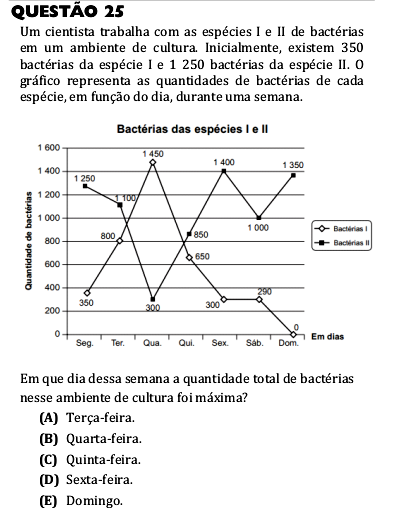
\includegraphics[width=10cm]{L1Q25.png}
	\end{center}
\end{figure}
\par\textbf{(Gabarito: A)} Queremos encontrar o dia em que a quantidade total de bactérias foi a maior, ou seja, o dia em que a soma das quantidades de bactérias de cada espécie foi a maior. Observando o gráfico, temos:
\begin{align*}
\text{Seg.: }1250+350 = 1600 \\
\text{Ter.: }1100+800 = 1900 \\
\text{Qua.: }1450+300 = 1750 \\
\text{Qui.: }850+650 = 1500 \\
\text{Sex.: }1400+300 = 1700 \\
\text{Sáb.: }1000+290 = 1250 \\
\text{Dom.: }1350+0 = 1350
\end{align*}
\par\vspace{0.3cm} Logo, o dia da semana com a maior quantidade total de bactérias foi Terça-feira.
\begin{figure}[H]
	\begin{center}
		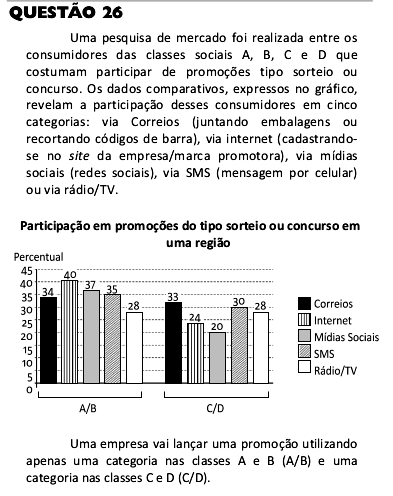
\includegraphics[width=9cm]{L1Q26_1.png}
	\end{center}
\end{figure}
\begin{figure}[H]
	\begin{center}
		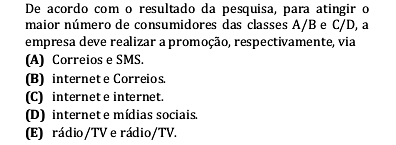
\includegraphics[width=9cm]{L1Q26_2.png}
	\end{center}
\end{figure}
\par\textbf{(Gabarito: B)} No gráfico das clases A/B, vemos que a internet é a mais usada. No gráfico das clases C/D, vemos que os Correios são mais utilizados. Logo, a empresa deve realizar a promoção via internet e Correios.
\begin{figure}[H]
	\begin{center}
		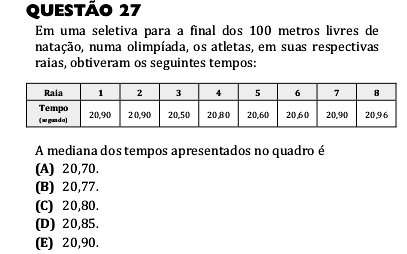
\includegraphics[width=10cm]{L1Q27.png}
	\end{center}
\end{figure}
\par\textbf{(Gabarito: D)} Colocando os dados em ordem crescente, temos:
\begin{equation*}
20,50; 20,60; 20,60; 20,80; 20,90; 20,90; 20,90; 20,96
\end{equation*}
\par\vspace{0.3cm} Como temos $8$ valores, a mediana será dada pela média aritmética do $4^\circ$ com o $5^\circ$ valor. Calculando, temos:
\begin{equation*}
\frac{20,80 + 20,90}{2} = 20,85
\end{equation*}
\begin{figure}[H]
	\begin{center}
		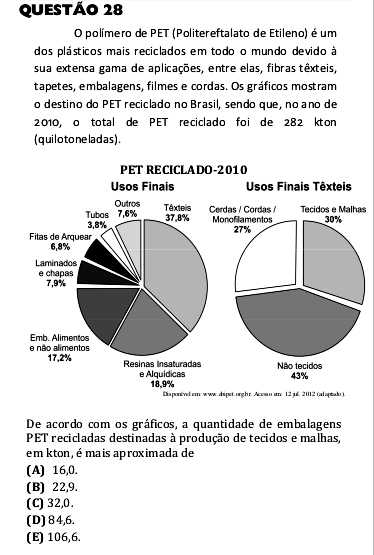
\includegraphics[width=10cm]{L1Q28.png}
	\end{center}
\end{figure}
\par\textbf{(Gabarito: C)} Dos dois gráficos, temos que a quantidade de embalagens PET recicladas destinadas à produção de tecidos e malhas é igual a
\begin{equation*}
30\%\times 37,8\%\times 282 = 31,9788 \approx 32\text{ kton}
\end{equation*}
\begin{figure}[H]
	\begin{center}
		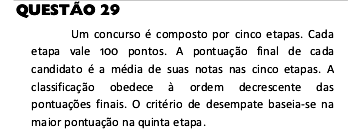
\includegraphics[width=10cm]{L1Q29_1.png}
	\end{center}
\end{figure}
\begin{figure}[H]
	\begin{center}
		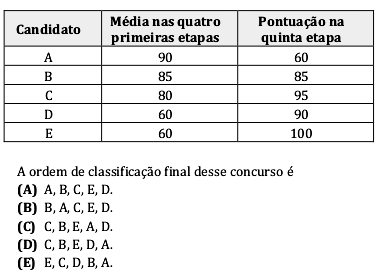
\includegraphics[width=10cm]{L1Q29_2.png}
	\end{center}
\end{figure}
\par\textbf{(Gabarito: B)} Queremos classificar os candidatos conforme suas médias nas cinco etapas do concurso. Para isso, podemos considerar apenas a soma das pontuações nas cinco etapas, pois quanto maior a soma, maior a média. 
\par\vspace{0.3cm} A segunda coluna da tabela nos dá as médias nas quatro primeiras etapas de cada candidato. Para descobrir a soma das pontuações nas quatro primeiras etapas, basta multiplicarmos esses valores por $4$, uma vez que a média é calculando fazendo-se a soma e dividindo por $4$. Assim, as somas das pontuações são as seguintes:
\begin{align*}
\text{Candidato A: }4\times 90 + 60 = 420 \\
\text{Candidato B: }4\times 85 + 85 = 425 \\
\text{Candidato C: }4\times 80 + 95 = 415 \\
\text{Candidato D: }4\times 60 + 90 = 330 \\
\text{Candidato E: }4\times 60 + 100 = 340 \\
\end{align*}
\par\vspace{0.3cm} Logo, a ordem final de classificação é B,A,C,E,D.

\section{Grandezas e medidas}
\begin{figure}[H]
	\begin{center}
		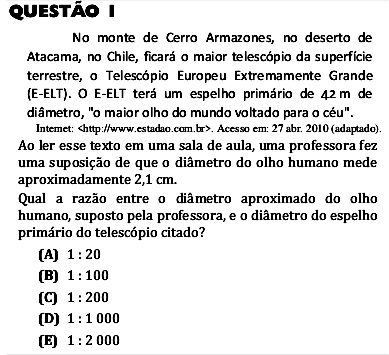
\includegraphics[width=10cm]{L2Q1.png}
	\end{center}
\end{figure}
\par\textbf{(Gabarito: E)} Do texto, o diâmetro do espelho do telescópio mede $42$ metros. Convertendo para centímetros, temos $4200$ centímetros. Portanto, a razão entre o diâmetro aproximado do olho e o diâmetro do espelho é
\begin{equation*}
\frac{2,1}{4200} = \frac{21}{42000} = \frac{1}{2000} = 1:2000
\end{equation*}
\begin{figure}[H]
	\begin{center}
		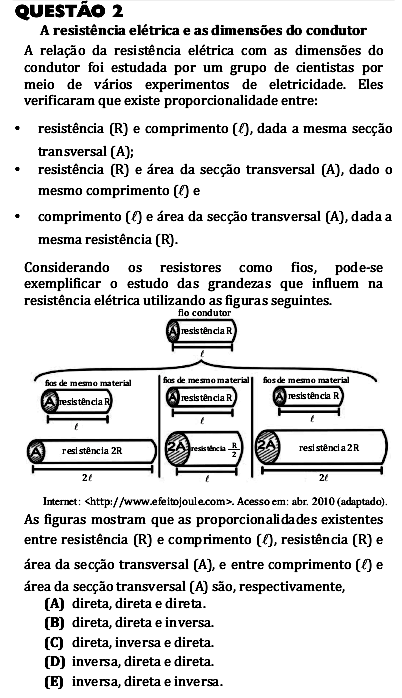
\includegraphics[width=10cm]{L2Q2.png}
	\end{center}
\end{figure}
\par\textbf{(Gabarito: C)} Do texto, podemos ver que quando o comprimento ($l$) dobra, a resistência ($R$) também dobra, logo $l$ e $R$ são diretamente proporcionais. Por outro lado, quando a área de secção transversal ($A$) dobra, a resistência ($R$) cai pela metade, logo $A$ e $R$ são inversamente proporcionais. Por fim, se mantivermos a mesma resistência, dobrar o comprimento ($l$) implica dobrar a área de secção transversal ($A$), logo $A$ e $l$ são diretamente proporcionais.
\begin{figure}[H]
	\begin{center}
		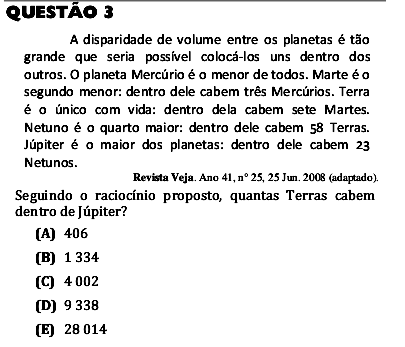
\includegraphics[width=11cm]{L2Q3.png}
	\end{center}
\end{figure}
\par\textbf{(Gabarito: B)} Do texto, sabemos que em Júpiter cabem $23$ Netunos e que, em cada Netuno, cabem $58$ Terras. Logo, em Júpiter cabem $23\times 58 = 1334$ Terras.
\begin{figure}[H]
	\begin{center}
		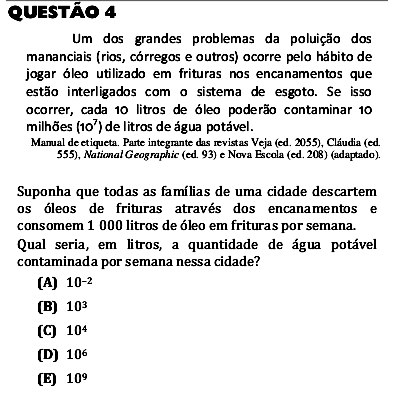
\includegraphics[width=10cm]{L2Q4.png}
	\end{center}
\end{figure}
\par\textbf{(Gabarito: E)} Do texto, sabemos que cada $10$ litros de óleo contaminam $10^7$ litros de água potável. Também do texto, sabemos que por semana são consumidos $1000$ litros de óleo. Como cada $10$ litros de óleo contaminam $10^7$ litros de água, temos a seguinte proporção:
\begin{equation*}
\frac{10}{10^7} = \frac{1000}{x} \iff 10x = 10^{10} \iff x = 10^9\text{ litros de água potável}
\end{equation*}
\begin{figure}[H]
	\begin{center}
		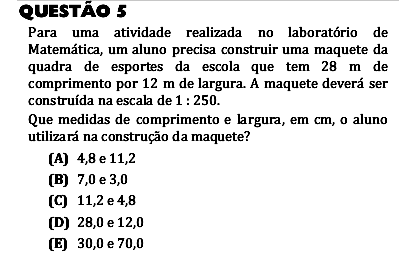
\includegraphics[width=11cm]{L2Q5.png}
	\end{center}
\end{figure}
\par\textbf{(Gabarito: C)} Do texto, sabemos que a escala da maquete é $1: 250$. Isso quer dizer que cada centímetro da maquete corresponde a $250$ centímetros na vida real. O comprimento da quadra é $28$ metros. Convertendo para centímetros, temos $2800$ centímetros. Usando a escala, temos a seguinte proporção:
\begin{equation*}
\frac{1}{250} = \frac{C}{2800} \iff 250C = 2800 \iff C = \frac{2800}{250} = 11,2\text{ centímetros}
\end{equation*}
\par\vspace{0.3cm} Portanto, o comprimento da quadra, na maquete, é de $11,2$ centímetros. Semelhantemente para a largura, temos:
\begin{equation*}
\frac{1}{250} = \frac{L}{1200} \iff 250L = 1200 \iff L = \frac{1200}{250} = 4,8\text{ centímetros}
\end{equation*}
\begin{figure}[H]
	\begin{center}
		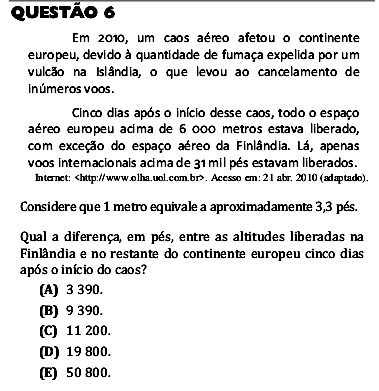
\includegraphics[width=10cm]{L2Q6.png}
	\end{center}
\end{figure}
\par\textbf{(Gabarito: C)} Do texto, sabemos que $1$ metro corresponde a $3,3$ pés. Daí, sabendo que a altitude liberada no continente europeu é de $6000$ metros, podemos converter esse valor para pés, obtendo:
\begin{equation*}
6000\times 3,3 = 19800 \text{ pés}
\end{equation*} 
\par\vspace{0.3cm} Do texto, a altitude liberada na Finlândia é de $31000$ pés. Logo, a diferença é de $31000 - 19800 = 11200$ pés.
\begin{figure}[H]
	\begin{center}
		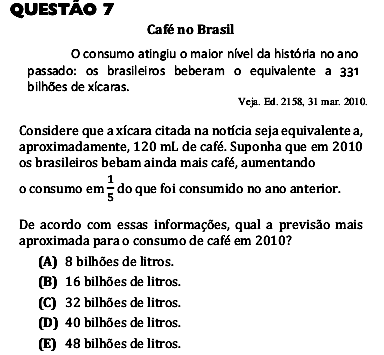
\includegraphics[width=9.5cm]{L2Q7.png}
	\end{center}
\end{figure}
\par\textbf{(Gabarito: E)} Do texto, sabemos que em $2009$ os brasileiros beberam $331\times 10^9$ xícaras de café. Como cada xícara tem $120$mL de café, segue que a quantidade de café ingerida em $2009$ foi de:
\begin{equation*}
331\times 10^9\times 120\times 10^{-3}\text{ L} =  39720\times 10^6\text{ L} = 39,72\times 10^9\text{ L}
\end{equation*}
\par\vspace{0.3cm} Por fim, considerando que o consumo aumenta em $\displaystyle{ \frac{1}{5} }$ em relação a $2009$, temos que o consumo em $2010$ será de:
\begin{equation*}
\left(39,72\times 10^9 + \frac{1}{5}\times 39,72\times 10^9\right)\text{ L} = \frac{6}{5}\times 39,72\times 10^9 = 47,664\times 10^9\approx 48\text{ bilhões de litros}
\end{equation*}
\begin{figure}[H]
	\begin{center}
		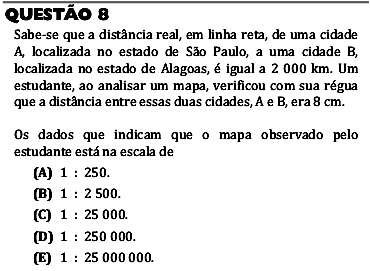
\includegraphics[width=9.5cm]{L2Q8.png}
	\end{center}
\end{figure}
\par\textbf{(Gabarito: E)} Do texto, sabemos que a distância real é de $2000$ km $= 200.000.000$ cm e que a distância na maquete é de $8$ cm. Daí, a escala é:
\begin{equation*}
\frac{8}{200.000.000} = \frac{1}{25.000.000} = 1:25.000.000
\end{equation*}
\begin{figure}[H]
	\begin{center}
		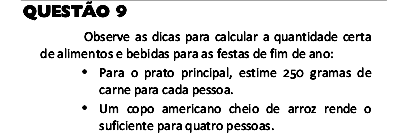
\includegraphics[width=9.5cm]{L2Q9_1.png}
	\end{center}
\end{figure}
\begin{figure}[H]
	\begin{center}
		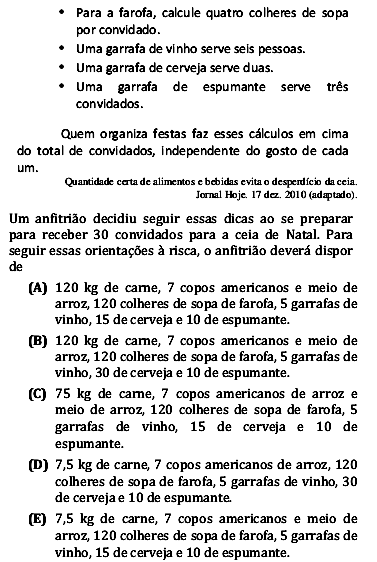
\includegraphics[width=9.5cm]{L2Q9_2.png}
	\end{center}
\end{figure}
\par\textbf{(Gabarito: E)} Do texto, sabemos que a estimativa é de $250$ gramas de carne por pessoa. Logo, para $30$ pessoas, devemos ter $30\times 250 = 7500$ gramas, ou seja, $7,5$ quilos de carne. 
\par\vspace{0.3cm} Cada copo americano de arroz serve quatro pessoas. Como $30\div4 = 7,5$, então para $30$ pessoas devemos ter $7,5$ copos americanos de arroz.
\par\vspace{0.3cm} Para a farofa, devemos ter $4$ colheres de sopa por convidado. Logo, para $30$ convidades, devemos ter $30\times4 = 120$ colheres de sopa de farofa.
\par\vspace{0.3cm} Cada garrafa de vinho serve $6$ pessoas. Logo, precisamos de $30\div6 = 5$ garrafas de vinho para servir as $30$ pessoas.
\par\vspace{0.3cm} Similarmente, cada garrafa de cerveja serve $2$ pessoas. Logo, precisamos de $30\div2 = 15$ garrafas de cerveja para servir as $30$ pessoas.
\par\vspace{0.3cm} Por fim, cada garrafa de espumante serve $3$ convidados. Logo, precisamos de $30\div3 = 10$ garrafas para servir todos os $30$ convidados.
\begin{figure}[H]
	\begin{center}
		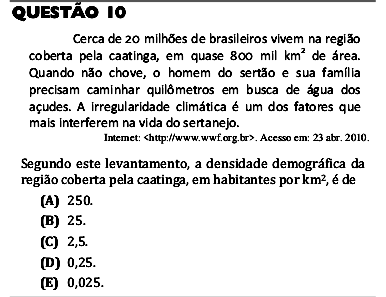
\includegraphics[width=9.5cm]{L2Q10.png}
	\end{center}
\end{figure}
\par\textbf{(Gabarito: B)} Do texto, sabemos que há uma população de $20\times 10^6$ habitantes, distribuídos em uma área de $800.000$ quilômetros quadrados. Logo, a densidade demográfica é:
\begin{equation*}
\frac{20\times 10^6}{800.000}\text{ habitantes/km$^2$} = \frac{20\times 10^6}{80\times 10^4}\text{ habitantes/km$^2$} = \frac{100}{4}\text{ habitantes/km$^2$} = 25\text{ habitantes/km$^2$}
\end{equation*}
\begin{figure}[H]
	\begin{center}
		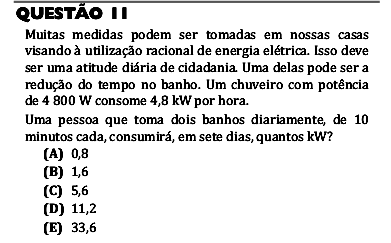
\includegraphics[width=10cm]{L2Q11.png}
	\end{center}
\end{figure}
\par\textbf{(Gabarito: D)} Considerando que a pessoa toma dois banhos por dia, cada um de $10$ minutos, então em uma semana o tempo total de banho é de $7\times 2\times 10 = 140$ minutos. 
Do texto, o chuveiro consome $4,8$ kW/hora, ou seja:
\begin{equation*}
\frac{4,8\text{kW}}{1\text{ hora}} = \frac{ 4,8\text{kW} }{ 60\text{ minutos} } = \frac{ 0,8\text{kW} }{ 10\text{ minutos} } = \frac{0,08\text{kW}}{1 \text{ minuto}}
\end{equation*}
\par\vspace{0.3cm} Portanto, como o chuveiro consome $0,08$ kW por minuto e, em $7$ dias o chuveiro é usado por $140$ minutos, o consumo total será de $140\times 0,08 = 11,2$ kW.
\begin{figure}[H]
	\begin{center}
		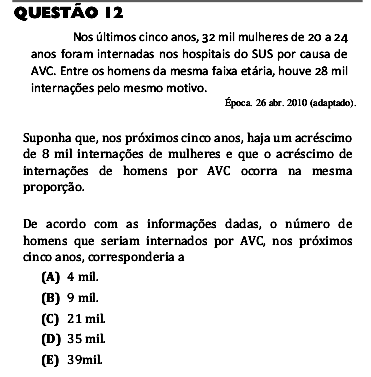
\includegraphics[width=9.5cm]{L2Q12.png}
	\end{center}
\end{figure}
\par\textbf{(Gabarito: D)} O acréscimo no número de internações de mulheres foi de $8$ mil. Proporcionalmente, isso corresponde a:
\begin{equation*}
\frac{8000}{32000} = \frac{8}{32} = \frac{1}{4} 
\end{equation*}
\par\vspace{0.3cm} ou seja, o acréscimo foi de $\displaystyle{\frac{1}{4}}$. Considerando que o aumento no número de internações de homens foi na mesma proporção, então o acréscimo foi de:
\begin{equation*}
\frac{1}{4}\times 28000 = 7000
\end{equation*}
\par\vspace{0.3cm} resultando em um total de $28000+7000 = 35000$ internações.
\begin{figure}[H]
	\begin{center}
		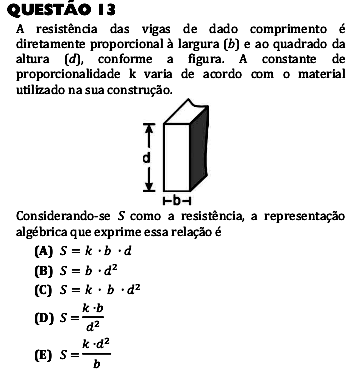
\includegraphics[width=8.2cm]{L2Q13.png}
	\end{center}
\end{figure}
\par\textbf{(Gabarito: C)} Do texto, sabemos que $S$ é diretamente proporcional a $b$ e diretamente proporcional a $d^2$, com constante de proporcionalidade $k$. Isso quer dizer que, mantendo $b$ fixo, $d^2$ e $S$ aumentam juntos na mesma proporção. De modo análogo, mantendo $d^2$ fixo, $b$ e $S$ também aumentam na mesma proporção. Analisando as opções, vemos que a única alternativa que satisfaz essas condições é $S = k\cdot b\cdot d^2$.
\begin{figure}[H]
	\begin{center}
		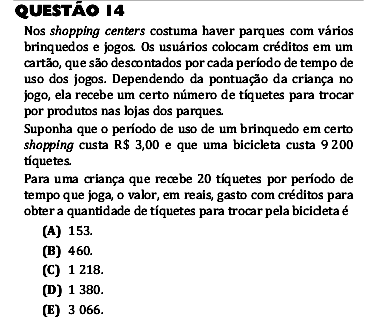
\includegraphics[width=9.5cm]{L2Q14.png}
	\end{center}
\end{figure}  
\par\textbf{(Gabarito: D)} Do texto, sabemos que são necessários $9200$ tíquetes para conseguir a bicicleta. Considerando que a criança consegue $20$ tíquetes por período, então são necessários $\displaystyle{ \frac{9200}{20} = 460 }$ períodos para conseguir a bicicleta. Como cada período custa $\text{R\$}3,00$, são necessários R\$$3,00\times 460 = \text{R\$}1380,00$.
\begin{figure}[H]
	\begin{center}
		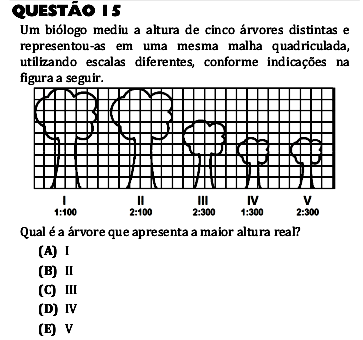
\includegraphics[width=10cm]{L2Q15.png}
	\end{center}
\end{figure}
\par\textbf{(Gabarito: D)} Utilizando a escala e a figura, podemos calcular a altura $h$ de cada árvore:
\begin{align*}
\text{I: } \frac{1}{100} = \frac{9}{h} &\iff h = 900\text{ cm} \\
\text{II: } \frac{2}{100} = \frac{9}{h} &\iff h = 450\text{ cm} \\
\text{III: } \frac{2}{300} = \frac{6}{h} &\iff h = 900\text{ cm} \\
\text{IV: } \frac{1}{300} = \frac{4,5}{h} &\iff h = 1350\text{ cm} \\
\text{V: } \frac{2}{300} = \frac{4,5}{h} &\iff h = 675\text{ cm} 
\end{align*}
\begin{figure}[H]
	\begin{center}
		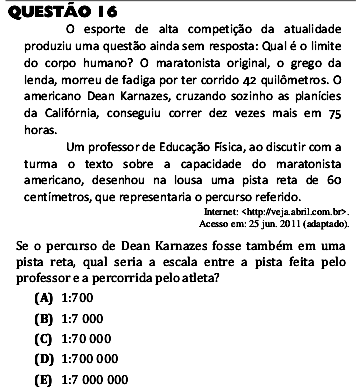
\includegraphics[width=9cm]{L2Q16.png}
	\end{center}
\end{figure}
\par\textbf{(Gabarito: D)} Sabemos que o percurso real é de $420$ km. Como, no quadro, essa distância corresponde a $60$ cm, temos a seguinte escala:
\begin{equation*}
\frac{60\text{ cm}}{420\text{ km}} = \frac{60\text{ cm}}{42.000.000\text{ cm}} = \frac{1}{700.000} = 1:700.000
\end{equation*}
\begin{figure}[H]
	\begin{center}
		\includegraphics[width=10cm]{L2Q17.png}
	\end{center}
\end{figure}
\par\textbf{(Gabarito: B)} Na primeira parte do trajeto, as laranjas foram divididas na proporção $6:5:4$. Isso quer dizer que cada um dos três levou as seguintes frações da quantidade $x$ de laranjas:
\begin{align*}
\text{José: }\frac{6}{6+5+4}\cdot x &= \frac{6}{15}\cdot x = \frac{2}{5}\cdot x \\
\text{Carlos: }\frac{5}{6+5+4}\cdot x &= \frac{5}{15}\cdot x = \frac{1}{3}\cdot x \\
\text{Paulo: }\frac{4}{6+5+4}\cdot x &= \frac{4}{15}\cdot x  
\end{align*}
\par\vspace{0.3cm} Na segunda parte do trajeto, temos a seguinte divisão:
\begin{align*}
\text{José: }\frac{4}{4+4+2}\cdot x = \frac{4}{10}\cdot x &= \frac{2}{5}\cdot x \\
\text{Carlos: }\frac{4}{4+4+2}\cdot x = \frac{4}{10}\cdot x &= \frac{2}{5}\cdot x \\
\text{Paulo: }\frac{2}{4+4+2}\cdot x = \frac{2}{10}\cdot x &= \frac{1}{5}\cdot x
\end{align*}
\par\vspace{0.3cm} Note que a fração das laranjas levadas por José não mudou de uma parte para a outra do trajeto; a parte de Carlos aumentou de $\displaystyle{ \frac{1}{3} }$ para $\displaystyle{ \frac{2}{5} }$ e a parte de Paulo diminuiu. Portanto, sabemos que Carlos levou $50$ laranjas a mais na segunda parte do trajeto. Com isso, temos a seguinte igualdade:
\begin{equation*}
\frac{1}{3}\cdot x + 50 = \frac{2}{5}\cdot x \iff \frac{2}{5}\cdot x - \frac{1}{3}\cdot x = 50 \iff \frac{1}{15}\cdot x = 50 \iff x = 750
\end{equation*}
\par\vspace{0.3cm} Portanto, a quantidade de laranjas transportadas na segunda parte do trajeto por José, Carlos e Paulo, respectivamente, foi $300$, $300$, $150$.
\begin{figure}[H]
	\begin{center}
		\includegraphics[width=10cm]{L2Q18.png}
	\end{center}
\end{figure}
\par\textbf{(Gabarito: B)} Vamos chamar de $A_i$ e $m_i$ a área da superfície corporal e a massa de um indivíduo na infância e de $A_m$ e $m_m$ a área de superfície corporal e a massa de um indivíduo na maturidade. Do texto, queremos obter $A_m$ em termos de $A_i$, sabendo que $m_m = 8m_i$. Usando a fórmula dada no texto, temos:
\begin{equation*}
A_m = k\cdot m_m^{2/3} = k\cdot (8m_i)^{2/3} = (2^3)^{2/3}k\cdot m^{2/3} = 4\cdot \underbrace{k\cdot m^{2/3}}_{A_i} = 4A_i
\end{equation*}
\par\vspace{0.3cm} Portanto, a área de superfície corporal é multiplicada por $4$.
\begin{figure}[H]
	\begin{center}
		\includegraphics[width=10cm]{L2Q19.png}
	\end{center}
\end{figure}
\par\textbf{(Gabarito: B)} Do texto, sabemos que $1^\circ$ ($1$ grau) equivale a $60'$ ($60$ minutos). Daí, podemos, através de uma proporção direta, converter $3'$ para graus da seguinte forma:
\begin{equation*}
\frac{1^\circ}{60'} = \frac{x}{3'} \iff x = \frac{3}{60} = \frac{1}{20} = 0,05^\circ
\end{equation*}
\par\vspace{0.3cm} Portanto, a representação angular da localização do vulcão é $124,05^\circ$.
\begin{figure}[H]
	\begin{center}
		\includegraphics[width=10cm]{L2Q20_1.png}
	\end{center}
\end{figure}
\begin{figure}[H]
	\begin{center}
		\includegraphics[width=4cm]{L2Q20_3.png}
	\end{center}
\end{figure}
\begin{figure}[H]
	\begin{center}
		\includegraphics[width=5cm]{L2Q20_2.png}
	\end{center}
\end{figure}
\par\textbf{(Gabarito: A)} Do texto, sabemos que, mantendo as outras dimensões constantes, a largura ($b$) e a resistência mecânica ($S$) aumentam na mesma proporção. O mesmo acontece para o quadrado da altura ($d^2$). Por fim, também sabemos que, mantendo as outras dimensões constantes, o quadrado do comprimento ($x^2$) diminui na mesma proporção que a resistência aumenta ($S$). Com isso, podemos deduzir que $S$ é expressa como:
\begin{equation*}
S = \frac{k\cdot b\cdot d^2}{x^2}
\end{equation*}
\begin{figure}[H]
	\begin{center}
		\includegraphics[width=10cm]{L2Q21.png}
	\end{center}
\end{figure}
\par\textbf{(Gabarito: D)} Da figura, podemos ver que a menor distância que o asteroide YU $55$ passou da superfície da Terra é de $325$ mil quilômetros. Podemos escrever esse valor da seguinte forma: $325000\text{ km} = 325\times 10^3\text{ km} = 3,25\times 10^5\text{ km}$.
\begin{figure}[H]
	\begin{center}
		\includegraphics[width=9.5cm]{L2Q22.png}
	\end{center}
\end{figure}
\par\textbf{(Gabarito: B)} Do texto, sabemos que a bacia não ecológica gasta $15$ litros por descarga, enquanto que a ecológica gasta apenas $6$. Também do texto, sabemos que a bacia não ecológica gasta $60$ litros por dia, ou seja, são dadas $60\div15 = 4$ descargas por dia. Se substituíssemos essa bacia por uma bacia ecológica, seriam gastos apenas $4\times 6 = 24$ litros por dia, resultando em uma economia de $60-24=36$ litros.
\begin{figure}[H]
	\begin{center}
		\includegraphics[width=10.5cm]{L2Q23.png}
	\end{center}
\end{figure}
\par\textbf{(Gabarito: A)} Do texto, sabemos que são necessárias $5$ gotas para cada $2$ kg de massa corporal. Se foram ministradas $30$ gotas de remédio, então a massa corporal é de $2\times(30\div5) = 2\times 6 = 12$ kg.
\begin{figure}[H]
	\begin{center}
		\includegraphics[width=10cm]{L2Q24.png}
	\end{center}
\end{figure}
\par\textbf{(Gabarito: D)} Do texto, sabemos que o cubo de $S$ é proporcional ao quadrado de $M$, ou seja:
\begin{equation*}
S^3 = k\cdot M^2 \iff S = \sqrt[3]{k\cdot M^2} = k^{\frac{1}{3}}\cdot M^{\frac{2}{3}}
\end{equation*}
\begin{figure}[H]
	\begin{center}
		\includegraphics[width=10.5cm]{L2Q25_1.png}
	\end{center}
\end{figure}
\begin{figure}[H]
	\begin{center}
		\includegraphics[width=4.5cm]{L2Q25_2.png}
	\end{center}
\end{figure}
\par\textbf{(Gabarito: B)} Do texto, sabemos que a força é dada pela expressão
\begin{equation*}
F = G\cdot\frac{m_1m_2}{d^2}
\end{equation*}
\par\vspace{0.3cm} Logo, podemos ver que a força ($F$) e o quadrado da distância ($d^2$) são inversamente proporcionais, isto é, a força diminui na mesma proporção que o quadrado da distância aumenta. Por isso, e como as massas são todas iguais, as maiores forças serão sentidas quanto mais próximo os satélites estiverem da Terra, resultando no gráfico do item B
\begin{figure}[H]
	\begin{center}
		\includegraphics[width=10cm]{L2Q26.png}
	\end{center}
\end{figure}.
\par\textbf{(Gabarito: A)} Queremos encontrar a razão entre as cadeiras coloridas de preto (reservadas) e o total de cadeiras. Contando, vemos que há $17$ cadeiras pretas de um total de $70$ cadeiras, resultando em uma razão de $\displaystyle{\frac{17}{70}}$.
\begin{figure}[H]
	\begin{center}
		\includegraphics[width=10cm]{L2Q27.png}
	\end{center}
\end{figure}
\par\textbf{(Gabarito: C)} Sabemos que $6$ ralos demoram $6$ horas para esvaziar um volume de $900$ m$^3$. Então, cada ralo, em $6$ horas, escoa um volume de $900\div6 = 150\text{ m}^3$, ou seja, cada ralo escoa $150\div6 = 25\text{ m}^3$ por hora. Logo, em $4$ horas, um ralo escoa $100\text{ m}^3$. Daí, para esvaziar um reservatório de $500$ m$^3$ em $4$ horas, serão necessários $500\div100 = 5$ ralos.
\begin{figure}[H]
	\begin{center}
		\includegraphics[width=10cm]{L2Q28.png}
	\end{center}
\end{figure}
\par\textbf{(Gabarito: B)} Do texto, sabemos que a fração de cimento presente no concreto é $\displaystyle{ \frac{1}{1+4+2} = \frac{1}{7} }$. Se a betoneira traz $14\text{ m}^3$ de concreto, então nessa carga haverá $\displaystyle{ \frac{1}{7}\cdot 14 = 2\text{ m}^3 }$ de cimento.
\begin{figure}[H]
	\begin{center}
		\includegraphics[width=10cm]{L2Q29.png}
	\end{center}
\end{figure}
\par\textbf{(Gabarito: D)} Vamos chamar de $T_i$ o peso de cada tijolo e $T_e$ o peso de cada telha. Do texto, sabemos que $1500$ telhas têm o mesmo peso que $1200$ tijolos, ou seja:
\begin{equation*}
1500T_e = 1200T_i \iff T_i = \frac{1500}{1200}\cdot T_e = \frac{15}{12}\cdot T_e = \frac{5}{4}\cdot T_e
\end{equation*}
\par\vspace{0.3cm} Então, cada tijolo pesa $1,25\times T_e$. Também do texto, o caminhão já está carregado com $900$ telhas, havendo espaço para mais $600$. Como cada tijolo pesa $1,25$ vezes o peso de cada telha, então a quantidade de tijolos que podem ser acrescentados à carga é, no máximo:
\begin{equation*}
\frac{600}{1,25} = \frac{600}{\frac{5}{4}} = \frac{2400}{5} = 480
\end{equation*}
\begin{figure}[H]
	\begin{center}
		\includegraphics[width=10cm]{L2Q30.png}
	\end{center}
\end{figure}
\par\textbf{(Gabarito: C)} Do texto, sabemos que a torneira ficou aberta durante $6$ horas. Considerando que cada hora tem $60$ minutos e cada minuto tem $60$ segundos, a quantidade de gotas desperdiçadas foi de
\begin{equation*}
\frac{6\times 60\times 60}{3} = 2\times 60 \times 60 = 7200
\end{equation*}
\par\vspace{0.3cm} Como cada gota tem $0,2$ mL, então o volume desperdiçado é de
\begin{equation*}
7200\times 0,2 \text{ mL} = 1440\text{ mL} = 1,44\text{ L}
\end{equation*}
\begin{figure}[H]
	\begin{center}
		\includegraphics[width=10cm]{L2Q31.png}
	\end{center}
\end{figure}
\par\textbf{(Gabarito: C)} Do texto, sabemos que o volume de uma lata de refrigerante é $355\text{ mL} = 35,5\text{ cL}$. Convertendo para onça fluida, temos:
\begin{equation*}
\frac{35,5}{2,95} \approxeq 12,034 \approx 12,03
\end{equation*}
\begin{figure}[H]
	\begin{center}
		\includegraphics[width=10cm]{L2Q32.png}
	\end{center}
\end{figure}
\par\textbf{(Gabarito: D)} Na figura, vemos que a escala linear foi ampliada de $1:25\ 000\ 000$ para $1: 4\ 000\ 000$. O fator de aumento é de
\begin{equation*}
\frac{\frac{1}{4\ 000\ 000}}{ \frac{1}{25\ 000\ 000} } = \frac{25\ 000\ 000}{4\ 000\ 000} = \frac{25}{4} = 6,25
\end{equation*}
\par\vspace{0.3cm} Note, entretanto, que queremos estimar o número de vezes que a \textbf{área} do estado foi ampliada. Por isso, é preciso elevar o fator de aumento ao quadrado, pois esse fator inicial é linear. Daí, obtemos que a área foi aumentada em
\begin{equation*}
(6,25)^2 = 39,0625
\end{equation*}
\par\vspace{0.3cm} valor que é maior que $30$ e menor que $40$.
\begin{figure}[H]
	\begin{center}
		\includegraphics[width=10cm]{L2Q33.png}
	\end{center}
\end{figure}
\par\textbf{(Gabarito: E)} Da figura, podemos ver que o aluno percorre $32$ quadradinhos, ida e volta, por dia. Logo, em $5$ dias, o aluno terá percorrido $160$ quadradinhos na figura. Usando a escala, temos:
\begin{equation*}
\frac{1}{25\ 000} = \frac{160}{x} \iff x = 160\times 25\ 000 = 4\ 000\ 000\text{ cm} = 40\ 000 \text{ m} = 40\text{ km}
\end{equation*}
\begin{figure}[H]
	\begin{center}
		\includegraphics[width=10cm]{L2Q34.png}
	\end{center}
\end{figure}
\par\textbf{(Gabarito: D)} Do texto, sabemos que as dimensões da base serão aumentadas em $25\%$, ou seja, $\displaystyle{ \frac{1}{4} }$. Logo, as novas medidas da base serão as medidas antigas multiplicadas por $\displaystyle{ 1 + \frac{1}{4} = \frac{5}{4} }$. Considerando que o volume da lata é dado pela área da base (que é um quadrado) vezes a altura, e chamando de $x$ o valor pelo qual devemos multiplicar a altura para que o volume não mude, temos que: 
\begin{equation*}
\frac{25}{16}\cdot l^2\cdot x\cdot h = l^2\cdot h \iff x = \frac{16}{25} = \frac{64}{100} = 64\%
\end{equation*}
\par\vspace{0.3cm} Portanto, a nova altura é igual a $64\%$ da antiga altura, havendo uma redução de $100\% - 64\% = 36\%$.
\begin{figure}[H]
	\begin{center}
		\includegraphics[width=10cm]{L2Q35.png}
	\end{center}
\end{figure}
\par\textbf{(Gabarito: D)} Vamos calcular as razões para cada jogador:
\begin{align*}
\text{Jogador I: }\frac{50}{85} = \frac{10}{17} &\approx 0,58 \\
\text{Jogador II: }\frac{40}{65} = \frac{8}{13} &\approx 0,61 \\
\text{Jogador III: }\frac{20}{65} = \frac{4}{13} &\approx 0,30 \\
\text{Jogador IV: }\frac{30}{40} = \frac{3}{4} &= 0,75\\
\text{Jogador V: }\frac{48}{90} = \frac{8}{15} &\approx 0,53 
\end{align*}
\par\vspace{0.3cm} Logo, podemos ver que o Jogador IV teve o melhor desempenho.
\begin{figure}[H]
	\begin{center}
		\includegraphics[width=10cm]{L2Q36.png}
	\end{center}
\end{figure}
\par\textbf{(Gabarito: E)} Podemos resolver de duas maneiras.
\paragraph{Opção (I):} Usando a escala, podemos converter as medidas do projeto para medidas reais. Como a escala é $1:100$, sabemos que cada centímetro no projeto representa $100$ centímetros na vida real. Portanto, as dimensões reais do armário são $300$ cm, $100$ cm e $200$ cm, resultando em um volume de $300\times 100\times 200 = 6\ 000\ 000$ cm$^3$.
\paragraph{Opção (II):} Podemos primeiro calcular o volume do armário no projeto e, depois, usar a escala para calcular o volume real. No projeto, o armário tem volume igual a $3\times 1 \times 2 = 6$ cm$^3$. Como a nossa escala linear é de $1:100$, então, para volumes, a escala é de $1: 100^3$, ou seja, $1:1\ 000\ 000$. Daí, o volume real do armário é igual a $6\times 1\ 000\ 000 = 6\ 000\ 000$ cm$^3$.
\begin{figure}[H]
	\begin{center}
		\includegraphics[width=9.5cm]{L2Q37.png}
	\end{center}
\end{figure}
\par\textbf{(Gabarito: D)} Vamos chamar a altura da porta inicial de $h_i$, a largura de $l_i$ e a espessura de $a_i$. O volume inicial da porta, ou seja, o volume de material usado inicialmente, é de
\begin{equation*}
V_i = l_i\cdot h_i\cdot a_i
\end{equation*} 
\par\vspace{0.3cm} Do texto, sabemos que a nova altura, $h_f$, é $\displaystyle{ \frac{1}{8} }$ maior que $h_i$, ou seja, $\displaystyle{ h_f = \frac{9}{8}\cdot h_i }$. Também sabemos que $a_f = a_i$. Queremos descobrir a razão entre $l_f$ e $l_i$. Para isso, vamos usar o fato de que o gasto de material é o mesmo, ou seja, os volumes são iguais. Isso nos dá a seguinte igualdade:
\begin{align*}
&V_i = V_f \\ 
&\iff l_i\cdot h_i\cdot a_i = l_f\cdot h_f \cdot a_f \\
&\iff l_i\cdot h_i \cdot a_i = l_f\cdot \frac{9}{8}\cdot h_i\cdot a_i \\
&\iff l_i\cdot \cancel{h_i \cdot a_i} = l_f\cdot \frac{9}{8}\cancel{\cdot h_i\cdot a_i} \\
&\iff  l_i = l_f\cdot \frac{9}{8} \\
&\iff \frac{l_f}{l_i} = \frac{8}{9}
\end{align*}
\begin{figure}[H]
	\begin{center}
		\includegraphics[width=10cm]{L2Q38.png}
	\end{center}
\end{figure}
\par\textbf{(Gabarito: A)} Do texto, as placas têm dimensões $6$ cm e $8$ cm. Logo, usando Pitágoras, o comprimento da diagonal é dado por
\begin{equation*}
d = \sqrt{6^2 + 8^2} = \sqrt{36+64} = \sqrt{100} = 10\text{ cm}
\end{equation*}
\par\vspace{0.3cm} Portanto, cada célula produz $24\times 10 = 240$ Wh por dia. Como o proprietário tem $100$ células, sua produção diária é de $24000$ Wh. Sabendo que sua residência consome $20160$ Wh e que ele quer que as placas produzam exatamente essa quantidade, é necessária uma queda de $24000 - 20160 = 3840$ Wh na produção. Como cada célula produz $240$ Wh por dia, é necessário retirar $3840\div 240 = 16$ células.
\begin{figure}[H]
	\begin{center}
		\includegraphics[width=10cm]{L2Q39_1.png}
	\end{center}
\end{figure}
\begin{figure}[H]
	\begin{center}
		\includegraphics[width=10cm]{L2Q39_2.png}
	\end{center}
\end{figure}
\par\textbf{(Gabarito: A)} Do texto, sabemos que os contêineres devem ser empilhados de modo a não sobrar espaços nem ultrapassar a área delimitada. Desse modo, os contêineres devem ser posicionados de modo que o comprimento fique paralelo ao maior lado da área de armazenamento, com $32$ metros. Desse modo, é possível colocar $32\div 6,4 = 5$ contêineres ao longo do maior lado da área. Além disso, é possível formar $10\div 2,5 = 4$ fileiras de cinco contêineres.
\par\vspace{0.3cm} Então, podemos colocar $20$ contêineres na base da nossa "pilha". Como temos $100$ contêineres para empilhar, serão necessários $5$ "camadas" de $20$ contêineres cada, resultando em uma altura total de $5\times 2,5 = 12,5$ metros.
\begin{figure}[H]
	\begin{center}
		\includegraphics[width=10cm]{L2Q40.png}
	\end{center}
\end{figure}
\par\textbf{(Gabarito: C)} A quantidade de soja exportada pelo Brasil em julho de $2012$ foi de $4,129\times 10^6$ toneladas. Como cada tonelada equivale a $1000$ quilos, essa quantidade é igual a $4,129\times 10^6\times 10^3 = 4,129\times 10^9$ quilogramas.
\begin{figure}[H]
	\begin{center}
		\includegraphics[width=10cm]{L2Q41.png}
	\end{center}
\end{figure}
\par\textbf{(Gabarito: B)} Vamos chamar de $I$ a idade da criança. Usando a "Fórmula de Young" para o medicamento Y, temos:
\begin{equation*}
14 = \frac{I}{I+12}\cdot 42 \iff \frac{I}{I+12} = \frac{14}{42} \iff \frac{I}{I+12} = \frac{1}{3} \iff I+12 = 3I \iff 2I = 12 \iff I = 6\text{ anos}
\end{equation*}
\par\vspace{0.3cm} Agora, usando a "Fórmula de Young" para o medicamento $X$, temos que a dosagem $d$ é igual a
\begin{equation*}
d = \frac{6}{18}\cdot 60 = \frac{1}{3}\cdot 60 = 20\text{ mg}
\end{equation*}
\begin{figure}[H]
	\begin{center}
		\includegraphics[width=10cm]{L2Q42.png}
	\end{center}
\end{figure}
\par\textbf{(Gabarito: E)} Queremos cortar as tábuas em tamanhos iguais, mas menor que $2\text{ m} = 200\text{ cm}$, ou seja, queremos encontrar o maior divisor comum de $540$, $810$ e $1080$ que seja menor que $200$. Para isso, vamos fatorar os três valores:
\begin{align*}
540 = 2^2\cdot 3^3\cdot 5\\
810 = 2\cdot 3^4\cdot 5\\
1080 = 2^3\cdot 3^3 \cdot 5
\end{align*} 
\par\vspace{0.3cm} Logo, o maior divisor comum de $540, 810$ e $1080$ é $2\cdot 3^3\cdot 5 = 270\text{ cm}$, que excede nosso limite. O maior divisor comum imediatamente inferior a esse é $3^3\cdot 5 = 135\text{ cm}$. Dividindo cada um dos comprimentos por esse valor, temos
\begin{align*}
540\div 135 = 4\\
810\div 135 = 6\\
1080\div 135 = 8
\end{align*}
\par\vspace{0.3cm} Logo, cada tábua de $540$ cm se torna $4$ tábuas de $135$ cm; cada tábua de $810$ cm se torna $6$ tábuas de $135$ cm; e cada tábua de $1080$ cm se torna $8$ tábuas de $135$ cm. Portanto, considerando a quantidade de tábuas de cada comprimento, o quantidade de peças produzidas é
\begin{equation*}
40\times 4 + 30\times 6 + 10\times 8 = 160+180+80 = 420
\end{equation*}
\begin{figure}[H]
	\begin{center}
		\includegraphics[width=9.5cm]{L2Q43.png}
	\end{center}
\end{figure}
\par\textbf{(Gabarito: A)} Do texto, sabemos que cada aplicação gasta $10$ unidades de insulina e antes de cada aplicação são descartadas $2$ unidades de insulina. Portanto, no processo de cada aplicação são gastas $12$ unidades de insulina, ou seja, $12\times 0,01 = 0,12\text{ mL}$. Como cada refil tem $3$ mL, então é possível fazer, no máximo, $3\div0,12 = 25$ aplicações por refil.
\begin{figure}[H]
	\begin{center}
		\includegraphics[width=9.5cm]{L2Q44.png}
	\end{center}
\end{figure}
\par\textbf{(Gabarito: D)} Do texto, o paciente deve tomar $1$ copo de $150$ mL a cada meia hora, ou seja, $2\times 150 = 300$ mL a cada hora. Como ele deve fazer isso durante $10$ horas, o volume total de água ingerida é $3000\text{ mL} = 3$ L. O único tipo de garrafa que satisfaz as condições de duas garrafas compradas e tomadas por inteiro é a Garrafa IV.
\begin{figure}[H]
	\begin{center}
		\includegraphics[width=9.5cm]{L2Q45.png}
	\end{center}
\end{figure}
\par\textbf{(Gabarito: C)} Fazendo as diferenças, temos
\begin{align*}
3,021 - 3 = 0,021 \\
3 - 2,96 = 0,040 \\
3 - 2,099 = 0,901 \\
3,07 - 3 = 0,07
\end{align*}
\par\vspace{0.3cm} Daí, vemos que a lente com espessura mais próxima é a com espessura de $3,021$ mm.
\begin{figure}[H]
	\begin{center}
		\includegraphics[width=9.5cm]{L2Q46.png}
	\end{center}
\end{figure}
\par\textbf{(Gabarito: B)} Do texto, sabemos que o felino pesa $3,0$ kg, tendo, portanto, $0,208$ m$^2$ de área de superfície corporal. Como, para cada metro quadrado, o felino deve receber $250$ mg, então a dose diária é igual a $250\times 0,208 = 52,0$ mg.
\begin{figure}[H]
	\begin{center}
		\includegraphics[width=9.5cm]{L2Q47.png}
	\end{center}
\end{figure}
\par\textbf{(Gabarito: E)} Como há $10$ pessoas na família e cada pessoa consome $0,08$ m$^3$ de água por dia, então o consumo diário total é igual a $10\times 0,08 = 0,8$ m$^3$. Durante $20$ dias, o consumo total será de $20\times 0,8 = 16$ m$^3$. Por fim, recorde que $1\text{ m}^3 = 1000\text{ L}$. Logo, o reservatório construído deve ter $16\text{ m}^3 = 16\ 000\text{ L}$.

\section{Porcentagem}
\begin{figure}[H]
	\begin{center}
		\includegraphics[width=10cm]{L3Q1.png}
	\end{center}
\end{figure}
\par\textbf{(Gabarito: C)} Para responder, basta notar que $\displaystyle{ 40\% = \frac{40}{100} = \frac{4}{10} = \frac{2}{5} }$. Logo, uma representação possível da situação é dividir o quadro em $5$ partes iguais e preencher $2$ delas.
\begin{figure}[H]
	\begin{center}
		\includegraphics[width=9.5cm]{L3Q2_1.png}
	\end{center}
\end{figure}
\begin{figure}[H]
	\begin{center}
		\includegraphics[width=10cm]{L3Q2_2.png}
	\end{center}
\end{figure}
\par\textbf{(Gabarito: A)} Do gráfico, a taxa de desempregados em Porto Alegre é de $9,8\%$. Considerando que o total de pessoas pesquisadas é $250\ 000$, então a quantidade de desempregados é $9,8\% \times 250\ 000 = 24\ 500$.
\begin{figure}[H]
	\begin{center}
		\includegraphics[width=9.5cm]{L3Q3.png}
	\end{center}
\end{figure}
\par\textbf{(Gabarito: D)} Na região Sudeste, $56\%$ dos estudantes entrevistados têm celular. Considerando que o total de entrevistados foi de $14\ 900$, então a quantidade de estudantes que têm celular é $56\% \times 14\ 900 = 8344$.
\begin{figure}[H]
	\begin{center}
		\includegraphics[width=9.5cm]{L3Q4_1.png}
	\end{center}
\end{figure}
\begin{figure}[H]
	\begin{center}
		\includegraphics[width=9.5cm]{L3Q4_2.png}
	\end{center}
\end{figure}
\par\textbf{(Gabarito: C)} Usando o gráfico, o desmatamento total foi de:
\begin{equation*}
4+136+326+549+766+797+3463+7293+10416 = 23750
\end{equation*} 
\par\vspace{0.3cm} Supondo que em $2009$ houve um aumento de $10,5\%$ em relação ao desmatamento em $2004$, então o desmatamento total em $2009$ é de
\begin{equation*}
1,105\times 23750 = 26243,75
\end{equation*}
\par\vspace{0.3cm} Fazendo a média entre os $9$ estados, obtemos que o desmatamenteo médio por estado em $2009$ é:
\begin{equation*}
\frac{262243,75}{9} \approx 2915,9\text{ km}^2
\end{equation*}
\par\vspace{0.3cm} valor que está entre $2800\text{ km}^2$ e $3200\text{ km}^2$.
\begin{figure}[H]
	\begin{center}
		\includegraphics[width=8cm]{L3Q5.png}
	\end{center}
\end{figure}
\par\textbf{(Gabarito: D)} A área total da página, em milímetros quadrados, é $400\times 260 = 104\ 000\text{ mm}^2$. Daí, $4\%$ dessa área é igual a $4\%\times 104\ 000 = 0,04\times 104\ 000 = 4160\text{ mm}^2$, ou seja, a região branca tem área de $4160$ milímetros quadrados.
Daí, temos
\begin{equation*}
x\cdot 26 = 4160 \iff x = \frac{4160}{26} = \frac{2080}{13} = 160\text{mm}
\end{equation*}
\begin{figure}[H]
	\begin{center}
		\includegraphics[width=10cm]{L3Q6.png}
	\end{center}
\end{figure}
\par\textbf{(Gabarito: C)} Do texto, o lucro da empresa aumentou de $\text{R\$}132\ 000,00$ para $\text{R\$}145\ 000,00$. Esse crescimento, em termos percentuais, é
\begin{equation*}
\frac{145\ 000}{132\ 000} = \frac{145}{132} \approx 1,09 \ (\text{crescimento de aproximadamente }1,09-1 = 0,09 = 9\%)
\end{equation*}
\par\vspace{0.3cm} ou seja, um bom desempenho.
\begin{figure}[H]
	\begin{center}
		\includegraphics[width=9.5cm]{L3Q7.png}
	\end{center}
\end{figure}
\par\textbf{(Gabarito: B)} Observe o diagrama abaixo:
\begin{center}
	\begin{forest}
	[$x$ [Curados: $40\%$ ][Não curados: $60\%$ [Tratamento inovador 1: $50\%$ [Curados: $35\%$] ] [Tratamento inovador 2: $50\%$ [Curados: $45\%$]  ] ] ]
	\end{forest}
\end{center}
\par\vspace{0.3cm} A partir daí, o total de pacientes curados por tratamentos inovadores é igual a
\begin{equation*}
35\%\cdot 50\%\cdot 60\%\cdot x + 45\%\cdot 50\%\cdot 60\%\cdot x = 80\%\cdot 50\%\cdot 60\% \cdot x = 40\%\cdot 60\%\cdot x = 24\%\cdot x
\end{equation*}
\begin{figure}[H]
	\begin{center}
		\includegraphics[width=9.5cm]{L3Q8.png}
	\end{center}
\end{figure}
\par\textbf{(Gabarito: C)} Do texto, a produção brasileira de etanol em $2006$ foi de $43\%\times 40\times 10^9\text{ L} = 17,2\times 10^9$ L, enquanto que a produção dos Estados Unidos foi de $45\%\times 40\times 10^9\text{ L} = 18\times 10^9$ L. Se a produção dos Estados Unidos, em $2009$, é apenas metade da produção de $2006$, então em $2009$ os Estados Unidos produzem $(18\times 10^9)\div2 = 9\times 10^9$ L.
\par\vspace{0.3cm} Por fim, considerando que a produção mundial se mantém em $40$ bilhões de litros em $2009$, então $88\%$ dessa quantidade é igual a $88\%\times 40\times 10^9 = 35,2\times 10^9$ L. Daí, temos que a produção brasileira, em $2009$, deve ser igual a $35,2\times 10^9 - 9\times 10^9 = 26,2\times 10^9$ L. Comparando com a produção de $2006$, temos
\begin{equation*}
\frac{26,2\times 10^9}{17,2\times 10^9} = \frac{26,2}{17,2} \approx 1,523 = 52,3\%
\end{equation*}
\begin{figure}[H]
	\begin{center}
		\includegraphics[width=9.5cm]{L3Q9.png}
	\end{center}
\end{figure}
\par\textbf{(Gabarito: C)} Vamos chamar de $x$ a quantia inicial aplicada. No primeiro mês, essa pessoa perdeu $30\%$ do investimento, ficando com $0,7x$. No segundo mês, ela recuperou $20\%$ do que havia perdido, ou seja, $20\%$ dos $30\%$ de $x$. Sabemos que depois desses dois meses, o montante era de $\text{R\$}3800,00$. Com isso, podemos montar a seguinte equação: 
\begin{equation*}
0,7x + 0,2\cdot 0,3x = 3800 \iff 0,76\cdot x = 3800 \iff x = 5000
\end{equation*}
\begin{figure}[H]
	\begin{center}
		\includegraphics[width=9.5cm]{L3Q10_1.png}
	\end{center}
\end{figure}
\begin{figure}[H]
	\begin{center}
		\includegraphics[width=9.5cm]{L3Q10_2.png}
	\end{center}
\end{figure}
\par\textbf{(Gabarito: D)} Vamos comparar os montantes de cada aplicação ao final de um mês:
\begin{align*}
\text{Poupança: }(1+0,56\%)\times 500 &= 1,0056\times 500 = \text{R\$}502,80 \\
\text{CDB: }(1+0,876\%)\times 500 - 4\%\times 0,876\%\times 500 &= (1,00876\times - 0,0003504)\times 500 = 1,0084096\times 500 = \text{R\$}504,2048  
\end{align*}
\par\vspace{0.3cm} Podemos ver que o CDB é a aplicação mais vantajosa, pois totaliza um montante de R\$$504,21$.
\begin{figure}[H]
	\begin{center}
		\includegraphics[width=9.5cm]{L3Q11.png}
	\end{center}
\end{figure}
\par\textbf{(Gabarito: C)} Vamos comparar as rentabilidades anuais. Para isso, vamos chamar de $x$ o investimento inicial para essas três aplicações. Daí, temos que ao final de $1$ ano os montantes de cada investimento serão iguais a:
\begin{align*}
&\text{Investimento A: }1,03^{12}x \approx 1,426x \\
&\text{Investimento B: }1,36x \\
&\text{Investimento C: }1,18^2x = 1,3924x
\end{align*}
\par\vspace{0.3cm} Com isso, vemos que o investimento A deve ser escolhido, pois sua rentabilidade anual é de $42,6\%$, sendo maior que as rentabilidades do investimento B ($36\%$) e do investimento C ($39,24\%$).
\begin{figure}[H]
	\begin{center}
		\includegraphics[width=9.5cm]{L3Q12_1.png}
	\end{center}
\end{figure}
\begin{figure}[H]
	\begin{center}
		\includegraphics[width=6cm]{L3Q12_3.png}
	\end{center}
\end{figure}
\begin{figure}[H]
	\begin{center}
		\includegraphics[width=6cm]{L3Q12_2.png}
	\end{center}
\end{figure}
\par\textbf{(Gabarito: C)} Olhando o gráfico, vemos que $25\%$ dos entrevistados responderam "NÃO". Considerando que o total de entrevistados é $279$, então a quantidade de entrevistados que responderam "NÃO" é $25\%\times 279 = 0,25\times 279 = 69,75$, valor que é maior que $50$ e menor que $75$.
\begin{figure}[H]
	\begin{center}
		\includegraphics[width=9.5cm]{L3Q13.png}
	\end{center}
\end{figure}
\par\textbf{(Gabarito: D)} Aqui, precisamos avaliar as opções para ver em qual delas Arthur consegue comprar o terreno e ficar com a maior quantidade de dinheiro. Vamos analisar opção por opção.
\paragraph{Opção 1.} Pagando à vista, Arthur compra o terreno mas não sobra nenhum dinheiro.
\paragraph{Opção 2.} Nessa opção, Arthur irá investir R\%$25000$ durante $6$ meses. Considerando que a aplicação rende $10\%$ ao semestre, então ao final do investimento Arthur terá $1,1\times 25000 = \text{R\$}27500$. Pagando a prestação de R\$$26000$, sobrarão ainda R\$$1500$.
\paragraph{Opção 3.} Nessa opção, Arthur irá investir R\$$35000$. Ao final do primeiro semestre, o montante será de $1,1\times 35000 = \text{R\$}38500$. Pagando a prestação de R\$$20000$, sobram R\$$18500$. Investindo esse valor por mais um semestre, Arthur terá $1,1\times 18500 = \text{R\$}20350$. Pagando a prestação de R\$$18000$, sobrarão ainda R\$$2350$.
\paragraph{Opção 4.} Nessa opção, Arthur irá investir R\$$40000$ durante um ano. Nesse caso, o montante ao final da aplicação será $1,1^2\times 40000 = \text{R\$}48400$. Pagando a prestação de R\$$39000$, sobrarão ainda R\$$9400$.
\paragraph{Opção 5.} Nessa opção, Arthur irá investir todo o valor de R\$$55000$ durante $1$ ano. Nesse caso, o montante ao final da aplicação será $1,1^2\times 55000 = \text{R\$}66550$. Pagando a prestação de R\$$60000$, sobrarão R\$$6550$.
\par\vspace{0.3cm} Portanto, a situação mais vantajosa é a opção 4.
\begin{figure}[H]
	\begin{center}
		\includegraphics[width=9.5cm]{L3Q14.png}
	\end{center}
\end{figure}
\par\textbf{(Gabarito: D)} Na primeira etapa, a taxa foi reduzida em $30\%$ e, na segunda, em $10\%$. Daí, temos que a taxa final é igual a
\begin{equation*}
(0,7\times 300)\times 0,9 = 0,63\times 300 = 189\text{ mg/dL}
\end{equation*}
\par\vspace{0.3cm} Portanto, o paciente está agora na categoria de diabetes melito.
\begin{figure}[H]
	\begin{center}
		\includegraphics[width=9.5cm]{L3Q15.png}
	\end{center}
\end{figure}
\par\textbf{(Gabarito: B)} O contribuinte em questão obteve um lucro de $\text{R\$}34000 - \text{R\$}26000 = \text{R\$}8000$. Do texto, sabemos que o imposto é de $15\%$ sobre o lucro. Logo, esse contribuinte deverá pagar $0,15\times 8000 = \text{R\$}1200$ de imposto.
\begin{figure}[H]
	\begin{center}
		\includegraphics[width=9.5cm]{L3Q16.png}
	\end{center}
\end{figure}
\par\textbf{(Gabarito: E)} Sem o cartão fidelidade, o cliente paga $0,8\times 50 = \text{R\$}40$. Com o cartão fidelidade, há um desconto adicional de $10\%$ sobre esse valor, ou seja, um desconto de $0,1\times 40 = \text{R\$}4$.
\begin{figure}[H]
	\begin{center}
		\includegraphics[width=9.5cm]{L3Q17.png}
	\end{center}
\end{figure}
\par\textbf{(Gabarito: D)} Vamos calcular o custo benefício de cada produto para os dois tipos.
\paragraph{Arroz}
\subparagraph{Tipo A.} O custo benefício é 
\begin{equation*}
\frac{\text{R\$}2}{1\text{ kg}} = \text{R\$}2/\text{kg}
\end{equation*}
\subparagraph{Tipo B.} O custo benefício é
\begin{equation*}
\frac{\text{R\$}1,7}{0,9\text{ kg}} = \frac{\text{R\$}17}{9\text{ kg}} < \text{R\$}2/\text{kg}
\end{equation*}
\par\vspace{0.3cm} Logo o tipo B deve ser escolhido para o arroz.
\paragraph{Feijão}
\subparagraph{Tipo A.} O custo benefício é
\begin{equation*}
\frac{\text{R\$}4,5}{1\text{ kg}} = \text{R\$}4,5/\text{kg}
\end{equation*}
\subparagraph{Tipo B.} O custo benefício é
\begin{equation*}
\frac{\text{R\$}4,1}{0,9\text{ kg}} = \frac{\text{R\$}41}{9} \approx \text{R\$}4,56/\text{kg} > \text{R\$}4,5/\text{kg} 
\end{equation*}
\par\vspace{0.3cm} Logo o tipo A deve ser escolhido para o feijão.
\paragraph{Soja}
\subparagraph{Tipo A.} O custo benefício é
\begin{equation*}
\text{R\$}3,8/\text{kg}
\end{equation*}
\subparagraph{Tipo B.} O custo benefício é
\begin{equation*}
\frac{\text{R\$}3,5}{0,9\text{ kg}} = \frac{\text{R\$}35}{9\text{ kg}} \approx \text{R\$}3,89/\text{kg} > \text{R\$}3,8/\text{kg}
\end{equation*}
\par\vspace{0.3cm} Logo o tipo A deve ser escolhido para a soja.
\paragraph{Milho}
\subparagraph{Tipo A.} O custo benefício é
\begin{equation*}
\text{R\$}6/\text{kg}
\end{equation*}
\subparagraph{Tipo B.} O custo benefício é
\begin{equation*}
\frac{\text{R\$}5,3}{0,9\text{ kg}} = \frac{\text{R\$}53}{9\text{ kg}} \approx \text{R\$}5,89/\text{kg} < \text{R\$}6/\text{kg}
\end{equation*}
\par\vspace{0.3cm} Logo o tipo B deve ser esoclhido para o milho.
\begin{figure}[H]
	\begin{center}
		\includegraphics[width=9.5cm]{L3Q18_1.png}
	\end{center}
\end{figure}
\begin{figure}[H]
	\begin{center}
		\includegraphics[width=9.5cm]{L3Q18_2.png}
	\end{center}
\end{figure}
\par\textbf{(Gabarito: C)} No caso de carga máxima, ou seja, $12$ toneladas, o ponto de sustentação central suporta $60\%\times 12 = 7,2$ toneladas (note que bastava calcular esse valor para podermos responder à questão, pois apenas uma das opções tem $7,2$ toneladas). Os outros pontos de sustentação recebem, cada um, $20\%$ da carga máxiam, ou seja, $20\%\times 12 = 2,4$ toneladas.
\begin{figure}[H]
	\begin{center}
		\includegraphics[width=9.5cm]{L3Q19.png}
	\end{center}
\end{figure}
\par\textbf{(Gabarito: E)} Do texto e do gráfico, sabemos que a taxa de desemprego total em dezembro de $2012$ é igual a $9\%$. Também sabemos que a taxa de desemprego oculto nesse mesmo perído é igual à metade do desemprego oculto em junho de $2012$, ou seja, igual a $2,2\div 2 = 1,1\%$. Como a taxa de desemprego total é dada pela soma da taxa de desemprego oculta com a taxa de desemprego aberto, temos que a taxa de desemprego aberto em dezembro de $2012$ é igual a $9 - 1,1 = 7,9\%$.
\begin{figure}[H]
	\begin{center}
		\includegraphics[width=9.5cm]{L3Q20.png}
	\end{center}
\end{figure}
\par\textbf{(Gabarito: C)} A variação percentual na taxa de fecundidade no período de $2000$ a $2010$ é igual a 
\begin{equation*}
\frac{1,9}{2,38} \approx 0,8
\end{equation*}
\par\vspace{0.3cm} Se essa taxa se mantiver para o período de $2010$ a $2020$, então em $2020$ a taxa de fecundidade será próxima de
\begin{equation*}
0,8\times 1,9 = 1,52
\end{equation*}
\begin{figure}[H]
	\begin{center}
		\includegraphics[width=9.5cm]{L3Q21_1.png}
	\end{center}
\end{figure}
\begin{figure}[H]
	\begin{center}
		\includegraphics[width=9.5cm]{L3Q21_2.png}
	\end{center}
\end{figure}
\par\textbf{(Gabarito: B)} Do texto, sabemos que as campanhas devem ser intensificadas nas regiões com percentuais de doadores por habitante iguais ou inferiores ao percentual do país. Olhando a tabela, vemos que a taxa de doadores por habitante no país é igual a $1,9\%$. Portanto, as campanhas devem ser intensificadas nas regiões com percentuais menores ou iguais a $1,9\%$. Olhando a tabela novamente, vemos que as regiões Norte, Nordeste e Sudeste têm percentuais menores ou iguais a $1,9\%$.
\begin{figure}[H]
	\begin{center}
		\includegraphics[width=10cm]{L3Q22.png}
	\end{center}
\end{figure}
\par\textbf{(Gabarito: B)} Do texto, sabemos que $8$ bilhões de litros de esgoto não são tratados, e isso corresponde, inicialmente, a $64\%$ do total de esgoto gerado. Chamando de $x$ a quantidade de esgoto gerado, temos que $0,64\times x = 8\times 10^9 \iff x = 12,5\times 10^9$ L. Portanto, são gerados $12,5$ bilhões de litros de esgoto. Supondo que a quantidade de esgoto não tratado passe a ser de $4$ bilhões de litros, isso corresponde a uma porcentagem de $\displaystyle{ \frac{4\times 10^9}{12,5\times 10^9} } = \frac{4}{12,5} = 0,32 = 32\%$. Portanto, a porcentagem de esgoto tratado será de $68\%$.	
\begin{figure}[H]
	\begin{center}
		\includegraphics[width=9.5cm]{L3Q23_1.png}
	\end{center}
\end{figure}
\begin{figure}[H]
	\begin{center}
		\includegraphics[width=9.5cm]{L3Q23_2.png}
	\end{center}
\end{figure}
\par\textbf{(Gabarito: D)} Do texto, sabemos que a área total do território brasileiro é de $853\times 10^6$ hectares e também que a área utilizada para a agricultura é de $80\times 10^6$ hectares. Daí, o percentual do território brasileiro utilizado para a agricultura é igual a
\begin{equation*}
\frac{80\times 10^6}{853\times 10^6} = \frac{80}{853} \approx 0,094 = 9,4\%
\end{equation*}
\begin{figure}[H]
	\begin{center}
		\includegraphics[width=9.5cm]{L3Q24.png}
	\end{center}
\end{figure}
\par\textbf{(Gabarito: C)} Sabendo que, em média, o brasileiro consome $200$ L de água por dia e que $15\%$ desse volume é destinado para demais atividades, então o volume, em litros, gasto nas demais atividades é de $15\%\times 200 = 30$ L. Adotando as sugestões de consumo e mantendo o mesmo gasto nas demais atividades, o consumo total, em litros, será de $24+18+3,2+2,4+22+30 = 99,6$ L, resultando em uma economia de $200 - 99,6 = 100,4$ L.
\begin{figure}[H]
	\begin{center}
		\includegraphics[width=9.5cm]{L3Q25.png}
	\end{center}
\end{figure}
\par\textbf{(Gabarito: A)} A menor quantidade de luz que atravessa o vidro e a película é $0,7\times 0,5 = 0,35 = 35\%$, enquanto que a maior quantidade de luz que atravessa o vidro e a película é $0,9\times 0,7 = 0,63 = 63\%$. Portanto, a transparência do vidro com a película varia no intervalo $[35;63]$.
\begin{figure}[H]
	\begin{center}
		\includegraphics[width=9.5cm]{L3Q26.png}
	\end{center}
\end{figure}
\par\textbf{(Gabarito: A)} Nessa questão, é importante notar que tomar a vacina e ela ser ineficaz é o mesmo que não tomar a vacina. Então, vamos chamar de $p$ a população de meninas e $x$ a porcentagem de meninas vacinadas. Então, há apenas duas maneiras de uma menina desenvolver o HPV: ou ela é vacinada mas a vacina não funciona; ou ela não é vacinada. Na primeira hipótese, a chance de desenvolver a doença é igual a $50\%\cdot 2\%\cdot x\cdot p$. Na segunda hipótese, a chance de desenvolver a doença é igual a $50\% \cdot (1-x)\cdot p$. A propabilidade total de desenvolver a doença será dada (pelo Princípio Fundamental da Contagem) pela soma das duas probabilidades citadas. Por fim, a nossa condição é que essa probabilidade total seja, no máximo, $5,9\%\cdot p$. Portanto, temos a seguinte desigualdade:
\begin{align*}
&50\%\cdot 2\% \cdot x\cdot p + 50\%\cdot (1-x)\cdot p \leq 5,9\%p \\ 
&\iff 50\%\cdot 2\% \cdot x\cdot \cancel{p} + 50\%\cdot (1-x)\cdot \cancel{p} \leq 5,9\%\cancel{p} \\
&\iff  0,01\cdot x + 0,5 - 0,5\cdot x \leq 0,059 \\
&\iff -0,49\cdot x \leq -0,441 \\
&\iff x\geq\frac{0,441}{0,49} = \frac{441}{490} = 0,9 = 90\%
\end{align*}
\par\vspace{0.3cm} Portanto, a menor quantidade de pessoas vacinadas que faz com que a probabilidade de desenvolver a doença seja no máximo $5,9\%$ é $90\%$. Logo, a proposta I deve ser implementada.
\begin{figure}[H]
	\begin{center}
		\includegraphics[width=9.5cm]{L3Q27.png}
	\end{center}
\end{figure}
\par\textbf{(Gabarito: E)} Os $10\%$ mais pobres, ou seja, $10\%\times 101,8 = 10,18$ milhões, ganham $1,1\%$ do total de rendimentos, ou seja, $1,1\%$ de $101,8\times 10^6\times 1202 = \text{R\$}122,3636\times 10^9$. Portanto, os $10\%$ mais pobres ganham $1,1\%\times 122,3636\times 10^9 = \text{R\$}1,3459996\times 10^9$. Daí, a renda média mensal dos $10\%$ mais pobres é 
\begin{equation*}
\frac{1,3459996\times 10^9}{10,18\times 10^6} = \frac{1345,9996}{10,18} = \text{R\$}132,22
\end{equation*}
\par\vspace{0.3cm} Por outro lado, os $10\%$ mais pobres (novamente, $10,18$ milhões de pessoas), ganham $44,5\%$ do total dos rendimentos, ou seja, $44,5\%\times 122,3636\times 10^9 = \text{R\$}54,451802\times 10^9$. Daí, a renda média mensal dos $10\%$ mais ricos é 
\begin{equation*}
\frac{54,451802\times 10^9}{10,18\times 10^6} = \frac{54451,802}{10,18} = \text{R\$}5348,90
\end{equation*}
\par\vspace{0.3cm} Portanto, a diferença é de $\text{R\$}5348,90 - \text{R\$}132,22 = \text{R\$}5216,68$.
\begin{figure}[H]
	\begin{center}
		\includegraphics[width=9.5cm]{L3Q28_1.png}
	\end{center}
\end{figure}
\begin{figure}[H]
	\begin{center}
		\includegraphics[width=9.5cm]{L3Q28_2.png}
	\end{center}
\end{figure}
\par\textbf{(Gabarito: A)} Pela figura, cada pequena seção quadrada da malha tem área $d^2$. Além disso, a área coberta pela malha é igual a $(d-1)^2$. Daí, o percentual coberto é 
\begin{equation*}
\displaystyle{ \frac{d^2 - (d-1)^2}{d^2} = \frac{d^2 - d^2+2d-1}{d^2} =  \frac{2d - 1}{d^2} }
\end{equation*}
\par\vspace{0.3cm} Queremos encontrar o valor de $d$ que faz com que a taxa de cobertura seja $75\%$, ou seja
\begin{align*}
\frac{2d-1}{d^2} = \frac{3}{4} &\iff 8d - 4 = 3d^2 \\
&\iff 3d^2 - 8d + 4 = 0 \\
&\iff d = \frac{8\pm\sqrt{64-48}}{6} \\
&\iff d = \frac{8\pm 4}{6} \\
&\iff d = 2 \ \text{ ou } \ d = \frac{2}{3}\text{ (não convém)}
\end{align*}
\par\vspace{0.3cm} em que a solução $d = 2/3$ é descartada pois teríamos $d - 1<0$, o que é absurdo.
\section{Geometria Plana}
\begin{figure}[H]
	\begin{center}
		\includegraphics[width=9.5cm]{L5Q1.png}
	\end{center}
\end{figure}
\par\textbf{(Gabarito: B)} A primeira encomenda tem quadros de $25\text{ cm}\times 50\text{ cm} = 1250\text{ cm}^2 = 0,125\text{ m}^2$ de área e molduras de perímetro $2\times 25 + 2\times 50 = 150\text{ cm} = 1,5\text{ m}$. Portanto, considerando que foram encomendados $8$ quadros, o valor da primeira encomenda é
\begin{equation*}
8\times ( 20\times 0,125 + 15\times 1,5 ) + 10 = 8\times (2,5 + 22,5) + 10 = 8\times 25 + 10 = \text{R\$}210
\end{equation*}
\par\vspace{0.3cm} Na segunda encomenda, cada quadro tem área de $50\times 100 = 5000\text{ cm}^2 = 0,5\text{ m}^2$ e perímetro de $2\times (50+100) = 300\text{ cm} = 3\text{ m}$. Portanto, considerando que foram encomendados $8$ quadros, o valor da segunda encomenda é
\begin{equation*}
8\times (20\times 0,5 + 15\times 3) + 10 = 8\times (10 + 45) + 10 = 8\times 55 + 10 = \text{R\$}450
\end{equation*}
\par\vspace{0.3cm} Vemos que o valor da segunda encomenda é maior que o valor da segunda encomenda, mas não o dobro (de fato, é maior que o dobro).
\begin{figure}[H]
	\begin{center}
		\includegraphics[width=10cm]{L5Q2.png}
	\end{center}
\end{figure}
\par\textbf{(Gabarito: C)} Vamos chamar de $x$ a altura em que se encontrava o balão. Da figura, vemos que
\begin{equation*}
\frac{x}{1,8} = \tan(60^\circ) \iff \frac{x}{1,8} = \sqrt{3} \iff x = 1,8\cdot\sqrt{3} \approxeq 1,8\cdot 1,73 = 3,114
\end{equation*}
\begin{figure}[H]
	\begin{center}
		\includegraphics[width=9.5cm]{L5Q3.png}
	\end{center}
\end{figure}
\par\textbf{(Gabarito: E)} Vamos chamar de $a$ o comprimento do lado $AC$ e $b$ o comprimento do lado $AB$. A área do triângulo $\triangle MNC$ é igual a $\displaystyle{ \frac{a}{2}\cdot\frac{b}{2}\cdot\frac{1}{2} = \frac{ab}{8} }$. A área da região sombreada pode ser calculada somando-se as áreas do triângulo $\triangle BPM$ com o retângulo $APMN$. Daí, a área sombreada tem área igual a $ \displaystyle{  \frac{b}{2}\cdot\frac{a}{2}\cdot\frac{1}{2} + \frac{a}{2}\cdot\frac{b}{2} = \frac{3ab}{8}  }  $, o triplo da área do triângulo $\triangle MNC$.
\begin{figure}[H]
	\begin{center}
		\includegraphics[width=9.5cm]{L5Q4.png}
	\end{center}
\end{figure}
\par\textbf{(Gabarito: B)} Traçe, a partir do centro da circunferência, raios $r$ com extremidade nos pontos de tangência. Chamando de $A$, $B$ e $C$ os vértices do triângulo retãngulo que circunscreve a circunferência (sendo $A$ o vértice que liga os lados de $6$ e $8$ cm e $B$ o vértice que liga os lados de $6$ e $10$ cm) e chamando de $O$ o centro da circunferência, obtemos três novos triângulos: $\triangle OAB$, $\triangle OBC$ e $\triangle OCA$. Note que as alturas de cada um desses novos triângulos é igual a $r$. Chamando de $S_{\triangle ABC}$ a área do triângulo $\triangle ABC$, temos que
\begin{equation*}
S_{\triangle ABC} = S_{\triangle OAB} + S_{\triangle OBC} + S_{\triangle OCA} \iff \frac{6\cdot 8}{2} = \frac{6\cdot r}{2} + \frac{10\cdot r}{2} + \frac{8\cdot r}{2} \iff 24 = 12\cdot r \iff r = 2\text{ cm}
\end{equation*}
\begin{figure}[H]
	\begin{center}
		\includegraphics[width=9.5cm]{L5Q5.png}
	\end{center}
\end{figure}
\par\textbf{(Gabarito: C)} Vamos calcular o perímetro e área de cada um dos terrenos. Para o terreno 1, temos:
\begin{align*}
\text{Perímetro: }2\times (55+45) &= 2\times 100 = 200\text{ m} \\
\text{Área: } 55\times 45 &= 2475\text{ m}^2
\end{align*}
\par\vspace{0.3cm} Para o terreno 2, temos:
\begin{align*}
\text{Perímetro: }2\times (55+55) &= 2\times 110 = 220\text{ m} \\
\text{Área: } 55\times 55 &= 3025\text{ m}^2
\end{align*}
\par\vspace{0.3cm} Para o terreno 3, temos:
\begin{align*}
\text{Perímetro: }2\times (60+30) &= 2\times 90 = 180\text{ m} \\
\text{Área: } 60\times 30 &= 1800\text{ m}^2
\end{align*}
\par\vspace{0.3cm} Para o terreno 4, temos:
\begin{align*}
\text{Perímetro: }2\times (70+20) &= 2\times 90 = 180\text{ m} \\
\text{Área: } 70\times 20 &= 1400\text{ m}^2
\end{align*}\par\vspace{0.3cm} Para o terreno 5, temos:
\begin{align*}
\text{Perímetro: }2\times (95+85) &= 2\times 180 = 360\text{ m} \\
\text{Área: } 95\times 85 &= 8075\text{ m}^2
\end{align*}
\par\vspace{0.3cm} Os únicos terrenos que atendem à restrição de no máximo $180$ m de perímetro são os terrenos $3$ e $4$. Desses dois, o com maior área é o 3.
\begin{figure}[H]
	\begin{center}
		\includegraphics[width=9.5cm]{L5Q6.png}
	\end{center}
\end{figure}
\par\textbf{(Gabarito: D)} Basta notar que rotacionando esse polígono por $120^\circ$, obtemos a mesma figura.
\begin{figure}[H]
	\begin{center}
		\includegraphics[width=10cm]{L5Q7_1.png}
	\end{center}
\end{figure}
\begin{figure}[H]
	\begin{center}
		\includegraphics[width=10cm]{L5Q7_2.png}
	\end{center}
\end{figure}
\par\textbf{(Gabarito: E)} Traçe a projeção perpendicular do ponto $P$ sobre a reta  definida por $A$ e $B$, e chame esse ponto de $P'$. Além disso, vamos chamar de $h$ a medida do segmento $\overline{PP'}$, que é altura do triângulo $\triangle APP'$. Note também que o triângulo $\triangle ABP$ é isósceles. Daí, o segmento $\overline{BP}$ tem medida igual a $2000$ m. Portanto, a partir do triângulo $\triangle BPP'$, temos que
\begin{equation*}
\cos(\alpha) = \frac{h}{2000} \iff \cos(30^\circ) = \frac{h}{2000} \iff \frac{\sqrt{3}}{2} = \frac{h}{2000} \iff h = 1000\sqrt{3}\text{ m}
\end{equation*}
\begin{figure}[H]
	\begin{center}
		\includegraphics[width=9cm]{L5Q8.png}
	\end{center}
\end{figure}
\par\textbf{(Gabarito: A)} Largando do mesmo ponto, o corredor da raia $1$ estaria sendo beneficiado, pois os corredores das raias mais externas percorreriam arcos de circunferências de raios maiores, percorrendo um perímetro mais longo.
\begin{figure}[H]
	\begin{center}
		\includegraphics[width=10cm]{L5Q9.png}
	\end{center}
\end{figure}
\par\textbf{(Gabarito: C)} Podemos ver que o caminho 
$$ K\to L\to G\to I\to J\to H\to F $$
\par\vspace{0.3cm} atende aos requisitos da questão.
\begin{figure}[H]
	\begin{center}
		\includegraphics[width=10cm]{L5Q10.png}
	\end{center}
\end{figure}
\par\textbf{(Gabarito: C)} Vamos calcular a área de cada ambiente. 
\begin{align*}
\text{Ambiente I: } 8\times 5 = 40\text{ m}^2 \text{ (modelo B)} \\
\text{Ambiente II: } 6\times 5 = 30\text{ m}^2 \text{ (modelo A)} \\
\text{Ambiente III: } 6\times 4 = 24\text{ m}^2 \text{ (modelo A)} \\
\text{Ambiente IV: } \frac{(6+4)\cdot 7}{2} = 35\text{ m}^2 \text{ (modelo B)} 
\end{align*}
\begin{figure}[H]
	\begin{center}
		\includegraphics[width=10cm]{L5Q11_1.png}
	\end{center}
\end{figure}
\begin{figure}[H]
	\begin{center}
		\includegraphics[width=10cm]{L5Q11_2.png}
	\end{center}
\end{figure}
\par\textbf{(Gabarito: B)} Do texto e da figura, sabemos que a base e a altura de cada um dos $4$ triângulos brancos medem, respectivamente, $0,25$ m e $0,5$ m. Daí, a área branca é dada por
\begin{equation*}
4\times \left( \frac{1}{4}\cdot\frac{1}{2}\cdot\frac{1}{2} \right) = \frac{1}{4}\text{ m}^2
\end{equation*}
\par\vspace{0.3cm} Como a área do quadrado é $1$ m$^2$, então a área sombreada é igual a
\begin{equation*}
1 - \frac{1}{4} = \frac{3}{4}\text{ m}^2
\end{equation*}
\par\vspace{0.3cm} Daí, o custo dos materiais é
\begin{equation*}
50\times \frac{1}{4} + 30\times\frac{3}{4} = 12,5+22,5 = \text{R\$}35,00
\end{equation*}
\begin{figure}[H]
	\begin{center}
		\includegraphics[width=10cm]{L5Q12.png}
	\end{center}
\end{figure}
\par\textbf{(Gabarito: E)} Na figura $1$, cada lado do losango tem medida igual a $2r$, sendo $r$ o raio das circunferências. Logo, o perímetro do losango na figura $1$ é $4\times 2r = 8r$. Na figura $2$, cada lado do losango tem medida igual a $3r$, sendo $r$ o raio das circunferências menores. Logo, o perímetro do losango na figura $2$ é $4\times 3r = 12r$. Daí, temos que a razão entre a nova área e a área antiga é
\begin{equation*}
\frac{12r}{8r} = \frac{12}{8} = \frac{3}{2} = 1,5
\end{equation*}
\par\vspace{0.3cm} Portanto, houve um aumento de $50\%$.
\begin{figure}[H]
	\begin{center}
		\includegraphics[width=10cm]{L5Q13.png}
	\end{center}
\end{figure}
\par\textbf{(Gabarito: A)} Aqui, temos uma circunferência de raio $R$ circunscrita em um quadrado de lado $L$. Para atender às exigências de segurança, o raio $R$ da circunferência tem de medir pelo menos metade da diagonal do quadrado, ou seja:
\begin{equation*}
R\geq \frac{L\sqrt{2}}{2} = \frac{L}{\sqrt{2}}
\end{equation*}
\begin{figure}[H]
	\begin{center}
		\includegraphics[width=10cm]{L5Q14.png}
	\end{center}
\end{figure}
\par\textbf{(Gabarito: E)} A área original é $3\times 5 = 15$. A área após a lavagem é $(5-x)(3-y) = 15 - 5y - 3x + xy$. Fazendo a diferença das duas, temos $15 - 15 + 5y + 3x - xy = 5y + 3x - xy$.
\begin{figure}[H]
	\begin{center}
		\includegraphics[width=10cm]{L5Q15.png}
	\end{center}
\end{figure}
\par\textbf{(Gabarito: A)} Inicialmente, as placas têm área $y^2$ cm$^2$ e cada caixa contém $N$ placas. Logo, a área máxima $S$ coberta pelas placas é $Ny^2$. Triplicando a medida dos lados das placas, cada uma terá área $9y^2$. A nova caixa contém $X$ placas, mas que ocupam a mesma área $S$ de antes. Logo, temos a igualdade:
\begin{equation*}
X\cdot 9y^2 = Ny^2 \iff X = \frac{N}{9}
\end{equation*}
\begin{figure}[H]
	\begin{center}
		\includegraphics[width=11cm]{L5Q16.png}
	\end{center}
\end{figure}
\par\textbf{(Gabarito: C)} O comprimento a ser cercado é $81+190+81 = 352$ metros. Como
\begin{equation*}
\frac{352}{48} = \frac{88}{12} = \frac{22}{3} = 7,33...
\end{equation*}
\par\vspace{0.3cm} é necessário comprar, pelo menos, $8$ rolos.
\begin{figure}[H]
	\begin{center}
		\includegraphics[width=8.5cm]{L5Q17.png}
	\end{center}
\end{figure}
\par\textbf{(Gabarito: E)} Analisando as figuras, vemos que a única que retrata corretamente a simetria em relação ao ponto $O$ é a opção "E".
\begin{figure}[H]
	\begin{center}
		\includegraphics[width=11cm]{L5Q18_1.png}
	\end{center}
\end{figure}
\begin{figure}[H]
	\begin{center}
		\includegraphics[width=11cm]{L5Q18_2.png}
	\end{center}
\end{figure}
\par\textbf{(Gabarito: C)} Vamos chamar a medida do segmento $\overline{AF}$ de $x$ e a medida do segmento $\overline{BF}$ de $y$. Note que $\triangle ABC \cong\triangle FBE$ e que $\triangle ABD\cong \triangle AFE$. Vamos chamar também de $h$ o comprimento da haste $EF$. Com isso, temos que:
\begin{equation*}
	\begin{cases}
		\displaystyle{ \frac{4}{h} = \frac{x+y}{y} } \\
		\displaystyle{ \frac{6}{h} = \frac{x+y}{x} }
	\end{cases} \iff \begin{cases}
	h = \displaystyle{\frac{4y}{x+y}} \\
	h = \displaystyle{\frac{6x}{x+y}}
	\end{cases} \iff 4y = 6x \iff y = \frac{3x}{2}
\end{equation*}
\par\vspace{0.3cm} Substituindo $y$ em termos de $x$ na primeira equação, temos que
\begin{equation*}
h = \frac{6x}{\frac{5x}{2}} = \frac{12}{5} = 2,4\text{ m}
\end{equation*} 
\begin{figure}[H]
	\begin{center}
		\includegraphics[width=10cm]{L5Q19.png}
	\end{center}
\end{figure}
\par\textbf{(Gabarito: A)} Chame de $x$ e $y$ as dimensões da base. Como cada dimensão sofre redução de $20\%$, então a área perdida é $20\%\cdot x\cdot 20\%\cdot y = 4\%\cdot xy$, ou seja, há uma redução de $4\%$.
\begin{figure}[H]
	\begin{center}
		\includegraphics[width=10cm]{L5Q20.png}
	\end{center}
\end{figure}
\par\textbf{(Gabarito: C)} Desenhe um triângulo conectando os centros das três circunferências internas. Note que esse triângulo é equilátero. Além disso, note que o segmento ligando um dos vértices desse triângulo ao seu centro mede $\displaystyle{\frac{2h}{3}}$, sendo $h$ a altura do triângulo, dada por $h = \frac{l\sqrt{3}}{2}$, com $l$ o lado do triângulo, nesse caso igual a $60$ cm. A seguir, note que o raio $R$ é igual ao segmento de medida $\displaystyle{\frac{2h}{3}}$ acrescido de $30+10 = 40$ cm (o raio da circunferência menor mais a margem de segurança). Portanto, temos que
\begin{equation*}
R = 40 + \frac{2h}{3} = 40 + \frac{2}{3}\cdot\frac{l\sqrt{3}}{2} = 40 + \frac{2}{3}\cdot 30\sqrt{3} = 40 + 20\sqrt{3} \approxeq 40 + 34 = 74\text{ cm}.
\end{equation*}
\begin{figure}[H]
	\begin{center}
		\includegraphics[width=10cm]{L5Q21.png}
	\end{center}
\end{figure}
\par\textbf{(Gabarito: D)} Note que a altura e largura disponíveis, na folha de papel, para reprodução da figura são $24$ cm e $36$ cm, respectivamente. Considerando que queremos aproveitar ao máximo a região disponível, considere as seguintes escalas:
\begin{align*}
\frac{24}{600} = \frac{4}{100} = \frac{1}{25} &= 1:25 \\
\frac{36}{800} = \frac{9}{200} = \frac{1}{22,222...} &= 1:22,222...
\end{align*}
\par\vspace{0.3cm} Qual escala devemos usar? Pelas alternativas, é claro que a primeira, mas existe um motivo melhor que esse. Note que calculamos cada uma dessas escalas considerando que todo a altura e toda a largura da folha, respectivamente, são aproveitadas. Por fim, note que usando a segunda escala para a altura, então o desenho teria uma altura de $600\div 22,222... = 27$, que excede o limite da folha de papel. Por outro lado, usando a primeira escala para a largura, então o desenho teria uma largura de $800\div25 = 32$, que não excede o limite da folha.
\begin{figure}[H]
	\begin{center}
		\includegraphics[width=10cm]{L5Q22_1.png}
	\end{center}
\end{figure} 
\begin{figure}[H]
	\begin{center}
		\includegraphics[width=10cm]{L5Q22_2.png}
	\end{center}
\end{figure}
\par\textbf{(Gabarito: C)} Primeiro, note que devido à condição de as mudas estarem à distância de pelo menos $3$ m das laterais, então na verdade a região disponível para colocarmos as mudas é um retângulo de lados $8$ m e $5,5$ m. Então, vamos colocar $3$ mudas em cada lado de maior comprimento: $A$, $B$ e $C$ de um lado e $D$, $E$, $F$ do outro. Já temos $6$. Agora, vamos posicionar $3$ sementes ao longo da mediatriz do lado menor do nosso retângulo. Essas novas sementes estarão nas interseções entre os segmentos $AE$ e $BD$, $BF$ e $CE$ e sobre o ponto médio do lado menor do retângulo. Temos $9$ sementes, mas precisamos garantir que as últimas $3$ realmente estão a $3$ metros das outras.
\par\vspace{0.3cm} Para isso, note que o triângulo $\triangle ABD$ é retângulo em $A$ e tem catetos com medidas $5,5$ m e $3$ m. Desse modo, sua hipotenusa $y$ tem medida:
\begin{equation*}
y = \sqrt{3^2 + 5,5^2} = \sqrt{9 + 30,25} > \sqrt{39} > 6\text{ m}
\end{equation*}
\par\vspace{0.3cm} Portanto, como a hipotenusa mede o dobro da distância entre as mudas, é claro que a distância entre elas é maior que $3$ m.

\begin{figure}[H]
	\begin{center}
		\includegraphics[width=10cm]{L5Q23.png}
	\end{center}
\end{figure}
\par\textbf{(Gabarito: A)} Recorde que a condição de existência para triângulos é que a soma de dois de seus lados seja sempre maior ou igual ao terceiro lado. No nosso caso, um dos lados mede $6$ palitos e sabemos que, somando todos os lados, temos $17$ palitos. Desse modo, temos, \textit{a priori}, as seguintes medidas para os lados:
\begin{align*}
6, 1, 8 \\
6, 2, 7 \\
6, 3, 6 \\
6, 4, 5
\end{align*}
\par\vspace{0.3cm} De todas essas configurações, a primeira é a única que não é possível, pois $6+1=7$ é menor que $8$. Portanto, podemos construir apenas $3$ triângulos.
\begin{figure}[H]
	\begin{center}
		\includegraphics[width=10cm]{L5Q24.png}
	\end{center}
\end{figure}
\par\textbf{(Gabarito: E)} Note que
\begin{equation*}
8\text{ hectares} = 8\text{ hm}^2 = 8\times 10^4\text{ m}^2 = 80\ 000\text{ m}^2
\end{equation*}

\begin{figure}[H]
	\begin{center}
		\includegraphics[width=10cm]{L5Q25.png}
	\end{center}
\end{figure}
\par\textbf{(Gabarito: A)} Nesse caso, queremos que o triângulo fique contido na circunferência. Vamos chamar de $R$ o raio da circunferência e $l$ o lado do triângulo equilátero. Para que a circunferência contenha o triângulo, devemos ter
\begin{equation*}
R\geq \frac{2h}{3}
\end{equation*}
\par\vspace{0.3cm} sendo $h$ a altura do triângulo. Como ele é equilátero, podemos substituir $h$ por $\displaystyle{ \frac{l\sqrt{3}}{2} }$, obtendo:
\begin{equation*}
R\geq \frac{2}{3}\cdot\frac{l\sqrt{3}}{2} = \frac{l\sqrt{3}}{3} = \frac{30\cdot 1,7}{3} = 17\text{ cm}
\end{equation*}
\par\vspace{0.3cm} Portanto, o tampo a ser escolhido é aquele com $18$ cm de raio.
\begin{figure}[H]
	\begin{center}
		\includegraphics[width=11cm]{L5Q26.png}
	\end{center}
\end{figure}
\par\textbf{(Gabarito: A)} A área original de cada garrafão é
\begin{equation*}
\frac{(600+360)\cdot 580}{2} = 278400\text{ cm}^2
\end{equation*}
\par\vspace{0.3cm} A nova área é
\begin{equation*}
490\cdot 580 = 284200\text{ cm}^2
\end{equation*}
\par\vspace{0.3cm} Comparando os dois valores, vemos que houve um aumento de $284200-278400 = 5800$ cm$^2$.
\begin{figure}[H]
	\begin{center}
		\includegraphics[width=9cm]{L5Q27_1.png}
	\end{center}
\end{figure}
\begin{figure}[H]
	\begin{center}
		\includegraphics[width=9cm]{L5Q27_2.png}
	\end{center}
\end{figure}
\par\textbf{(Gabarito: C)} Para o triângulo, note que usando semelhança entre o triângulo menor das proteínas e o triângulo todo, obtemos que a área correspondente às proteínas é $1/3$ da área total, ou seja, cerca de $33\%$, não atendendo às condições.
\par\vspace{0.3cm} Para o losango, note que os carboidratos ocupam $50\%$ da área, não atendendo às condições.
\par\vspace{0.3cm} Para o hexágono, note que as gorduras ocupam $2/6$ da área, ou seja, cerca de $33\%$, não atendendo às condições.
\par\vspace{0.3cm} Para o octógono, note que as proteínas ocupam $1/16$ da área, ou seja, $6,25\%$, não atendendo às condições.
\par\vspace{0.3cm} Resta, então, o pentágono, que de fato satisfaz as condições: os carboidratos ocupam $3/5 = 60\%$ da área, as proteínas, $1/10 = 10\%$ e as gorduras, $3/10 = 30\%$.
\begin{figure}[H]
	\begin{center}
		\includegraphics[width=11cm]{L5Q28.png}
	\end{center}
\end{figure}
\par\textbf{(Gabarito: A)} A cobertura com as antenas antigas era de
\begin{equation*}
2\cdot \pi\cdot 2^2 = 8\pi \text{ km}^2
\end{equation*}
\par\vspace{0.3cm} A nova antena tem cobertura de raio igual a $4$ km. Logo, a nova área de cobertura é igual a 
\begin{equation*}
\pi\cdot 4^2 = 16\pi \text{ km}^2
\end{equation*}
\par\vspace{0.3cm} Podemos ver que a área foi ampliada em $8\pi$ km$^2$.
\begin{figure}[H]
	\begin{center}
		\includegraphics[width=10cm]{L5Q29.png}
	\end{center}
\end{figure}
\par\textbf{(Gabarito: E)} Para visualizar a bandeirinha, basta refletir o polígono $MNOGD$ em torno do segmento $GO$. Fazendo isso, obtemos o desenho do item "E".

\end{document}